% Unified lychee manuscript — compile with xelatex
\documentclass[11pt]{article}

\usepackage[margin=1in]{geometry}
\usepackage{fontspec}
\setmainfont{Times New Roman}
\usepackage{graphicx}
\usepackage{booktabs}
\usepackage{array}
\usepackage{caption}
\usepackage{setspace}
\usepackage[hidelinks]{hyperref}
\usepackage{enumitem}
\usepackage{microtype}

\captionsetup{font=small,labelfont=bf,width=0.94\textwidth}
\setlength{\parskip}{0.35em}
\setlength{\parindent}{1.2em}
\emergencystretch=1.5em
\graphicspath{{figures/}{../../../results/figures/}}

\newcommand{\Pl}{\textit{P.~litchii}}
\newcommand{\q}{\textit{q}}

\title{\bfseries A registered genome-wide analysis identifies robust, context-dependent transcriptional responses of lychee to \textit{Peronophythora litchii}}
\author{Eric Zhuang}
\date{}

\begin{document}
\maketitle

\begin{abstract}
\noindent
Litchi downy blight, caused by the oomycete \textit{Peronophythora litchii}, severely damages lychee (\textit{Litchi chinensis} Sonn.). Public RNA-seq cohorts spanning cultivars, tissues, and infection times can resolve host responses and prioritize resistance candidates. We integrated five such cohorts in a two-stage analysis of the lychee--\Pl{} interaction. An exploratory reanalysis of Guiwei and Yurong1 leaves (GSE201243/PRJNA830488) identified 17 and 117 infection-responsive genes, respectively, and nominated 18 defense-associated candidates. We then prospectively registered genome-wide discovery and cross-context evaluation. Cultivar-by-infection analysis of 19,445 expressed genes identified 262 statistical candidates; 206 passed uniform mapping and gene-model quality control, 19 were significant under both DESeq2 and edgeR genome-wide analyses, and 16 passed the complete registered robustness procedure. Evidence integration prioritized 12 internally robust genes spanning carbohydrate and cell-wall remodeling, membrane and lipid transport, chaperone regulation, RNA metabolism, and specialized metabolism. In an independent pericarp time course contrasting susceptible and resistant cultivars (PRJNA450886), alpha-xylosidase LITCHI005518 and LITCHI001963 showed cross-context support. A 206-gene signature distinguished infection responses across tissues, with a significant leaf--fruit interaction demonstrating tissue and temporal dependence. Estimand-aligned follow-up confirmed infection responsiveness for 13 of 18 exploratory candidates in Guiwei and 16 of 18 in Yurong1, while the genome-wide interaction analysis refined their interpretation as within-cultivar rather than cultivar-differential responses. This analysis provides a prioritized candidate set, highlights cell-wall and carbohydrate processes, and defines contexts for experimental evaluation.

\vspace{0.6em}
\noindent\textbf{Keywords:} \textit{Litchi chinensis}; \textit{Peronophythora litchii}; downy blight; RNA-seq; cultivar-by-infection interaction; preregistered analysis; cross-context evaluation
\end{abstract}

\section{Introduction}

Lychee (\textit{Litchi chinensis} Sonn.) is a subtropical fruit crop of substantial economic importance in southern China, Southeast Asia, and a growing set of production regions worldwide [1]. Among its diseases, litchi downy blight, caused by the oomycete \textit{Peronophythora litchii} (historically also treated as \textit{Phytophthora litchii} [2]), is particularly damaging: the pathogen attacks young leaves, inflorescences, and fruit, produces water-soaked brown lesions, and drives severe postharvest decay [2,3]. Because chemical control is costly and resistance breeding depends on understanding how host genotypes differ in their response to infection, the molecular basis of cultivar-level variation in the response to \Pl{} is a question of both agronomic and biological interest.

The resources needed to address this question computationally have accumulated rapidly. High-quality genome assemblies are available for lychee [4], and several groups have profiled the transcriptional response to \Pl{} infection. Sun et al.\ compared a susceptible and a resistant cultivar across a pericarp infection time course and reported that the two genotypes deploy distinct early response programs [5]. Liu et al.\ described calcium-dependent protein kinase (LcCDPK) family members induced by \Pl{} inoculation [6], and Li et al.\ showed that the pathogen RXLR effector PlAvh202 promotes virulence by destabilizing a host ethylene-biosynthesis enzyme [7]. A pathogen-side transcriptome catalogued the \Pl{} pathogenicity arsenal [2]. In parallel, public repositories now hold RNA-seq series covering resistant and susceptible cultivars, leaf and fruit tissues, messenger and small RNA, and multiple time points. These series offer an opportunity, in principle, to distinguish genome-wide cultivar-dependent infection responses from responses common to all genotypes.

Realizing that opportunity requires an analysis matched to the biological question. The cultivar-by-infection interaction measures the difference between infection responses across genotypes and is distinct from differential expression within either cultivar. Because interaction effects are estimated with less precision than main effects, the deposited designs are small (typically three libraries per cultivar--treatment cell), and a genome-wide search requires explicit multiplicity control, candidate prioritization benefits from complementary statistical frameworks, mapping checks, and evaluation across independent cohorts. Applying these elements can distinguish broadly responsive genes from cultivar-dependent responses and define the contexts in which candidate expression patterns are most reproducible.

The first stage of the present work was an exploratory reanalysis of the GSE201243 leaf series [8] (Guiwei and Yurong1, mock versus inoculated, 24~h post-inoculation). It identified 17 significant infection-responsive genes in Guiwei and 117 in Yurong1, prioritized 18 candidates with defense-plausible annotations (among them jacalin-like lectin, pathogenesis-related and thaumatin/osmotin-like proteins, a heat-shock protein, lipid-transfer proteins, and calcium-binding proteins), and identified stress- and hormone-associated \textit{cis}-regulatory elements enriched relative to a randomized background. This hypothesis-generating stage created a focused set for a more comprehensive analysis: a genome-wide interaction test with false-discovery-rate control, evaluation in independent cohorts, and promoter analysis against biologically matched genomic backgrounds.

This paper presents that complete analytical arc. We prospectively registered a discovery and external-evaluation protocol that fixed dataset roles, models, thresholds, empty-result behavior, and evidence vocabulary before any external outcome was opened. Because every cohort is public, the staged unlock is a workflow-enforced computational safeguard rather than experimental blinding, and the chronology is documented in the Methods. Within the prespecified discovery cohort we fitted a genome-wide negative-binomial interaction model, applied uniform mapping and gene-model quality control, and assessed candidates using independent quantification, an alternative statistical framework, filter sensitivity, and leave-one-library-out refits. We then evaluated the frozen candidates (throughout, \emph{frozen} denotes a computed result fixed at a recorded checkpoint and not modified afterward), pathways, and a signed expression signature in independent public cohorts with roles fixed in advance. Separate annotation, promoter, small-RNA, and literature evidence classes were combined through a deterministic tier system. The resulting resource prioritizes robust candidates for lychee downy blight, resolves tissue- and time-dependent response patterns, and provides an explicit bridge from public transcriptomes to targeted experimental studies.

\section{Results}

\subsection{A two-stage design with prespecified dataset roles}

The study comprises an exploratory stage completed first and a confirmatory stage whose protocol was registered before its analyses began (Figure~\ref{fig:design}A; Table~\ref{tab:roles}). Five public cohorts enter the confirmatory stage in fixed, non-interchangeable roles. PRJNA830488 (GSE201243), the leaf series for Guiwei and Yurong1 at 24~h, is the sole discovery cohort; it is also the dataset analyzed in the exploratory stage. PRJNA450886, a pericarp time course contrasting the susceptible cultivar Guiwei with the resistant cultivar Heiye at 6, 24, and 48~h [5], serves as the primary external evaluation. Because it differs from the discovery cohort in tissue, resistant comparator, and time structure, we describe positive outcomes in it as \emph{cross-context support} rather than replication. PRJNA922966 (Feizixiao leaf and fruit, mock versus infected) tests generic infection-response transfer but cannot address the cultivar interaction; PRJNA922965 provides small-RNA libraries as an orthogonal modality; and PRJNA1090613 (Guiwei versus SFZ leaf) is exploratory only, because its time and resistance metadata could not be resolved. Under the registered firewall, no external outcome could alter the frozen discovery membership, signature weights, or thresholds, and the protocol explicitly allowed the top evidence tier to be empty.

\begin{figure}[p]
\centering
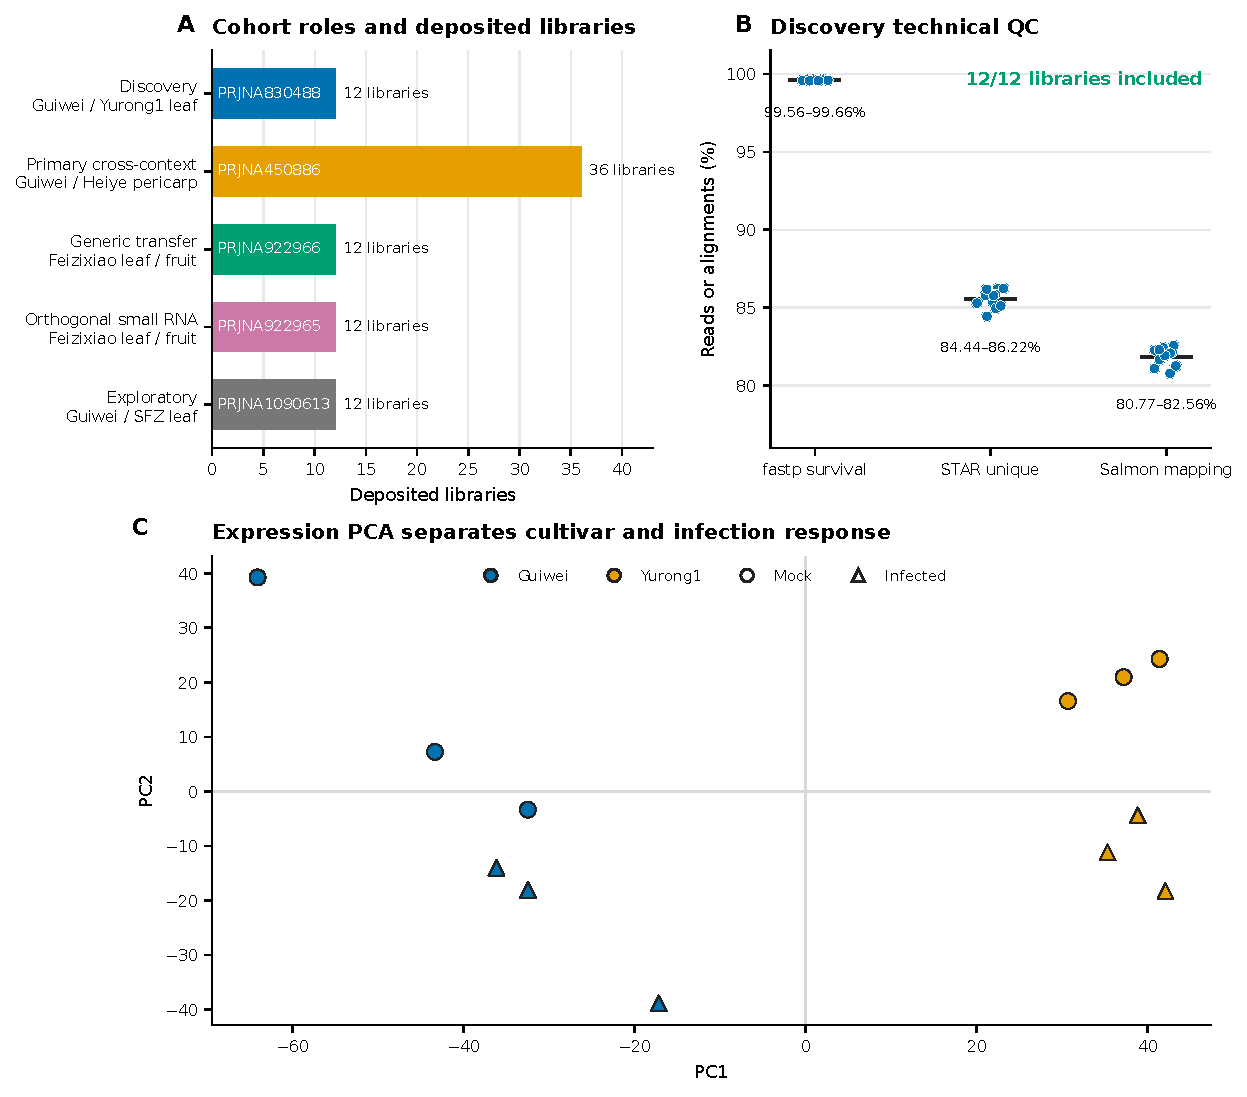
\includegraphics[width=0.98\textwidth]{figure1_study_design_qc.pdf}
\caption{\textbf{Study cohorts, discovery quality control, and expression structure.} (A) The five public cohorts with prespecified roles and deposited library counts. (B) Per-library technical quality in the discovery cohort: fastp read survival, STAR unique-alignment rate, and Salmon mapping rate; all 12 libraries passed the fixed inclusion gates. (C) Principal-component analysis of the discovery libraries separates cultivar and infection status.}
\label{fig:design}
\end{figure}

\begin{table}[t]
\centering
\caption{\textbf{Locked dataset roles and eligibility.}}
\label{tab:roles}
\small
\begin{tabular}{@{}p{3.2cm}p{5.6cm}p{3.3cm}p{2.6cm}@{}}
\toprule
\textbf{Accession} & \textbf{Design} & \textbf{Locked role} & \textbf{Evidence class} \\
\midrule
PRJNA830488 (GSE201243) & Guiwei/Yurong1 leaf; mock/infected; 24 h; 3 libraries per cell & Discovery & Conditional inferential \\
PRJNA450886 & Guiwei/Heiye pericarp; mock/infected; 6, 24, 48 h; 3 libraries per cell & Primary external evaluation & Cross-context \\
PRJNA922966 (GSE222651) & Feizixiao leaf/fruit; mock/infected; 24 h; 3 libraries per cell & Generic infection transfer & Cross-context \\
PRJNA922965 (GSE222650) & Feizixiao leaf/fruit small RNA; mock/infected; 24 h; 3 libraries per cell & Orthogonal modality & Orthogonal \\
PRJNA1090613 (GSE262200) & Guiwei/SFZ leaf; mock/infected; 3 libraries per cell & Exploratory only & Exploratory \\
\bottomrule
\end{tabular}
\end{table}

\subsection{Stage 1: exploratory candidate discovery in GSE201243}

The exploratory stage analyzed the 12 discovery libraries with per-cultivar differential-expression contrasts (infected versus mock) and identified 17 significant genes in Guiwei (15 up-regulated, 2 down-regulated) and 117 in Yurong1 (39 up-regulated, 78 down-regulated) at Benjamini--Hochberg adjusted $P<0.05$, suggesting a broader transcriptional response in Yurong1. From these lists, 18 genes were prioritized by combining statistical significance in at least one cultivar, large infection-associated fold changes, and annotations plausibly related to defense: among them a jacalin-like lectin (LITCHI028104), a pathogenesis-related protein (LITCHI011394), osmotin/thaumatin-like proteins (LITCHI009301, LITCHI002793), an HSP70-family chaperone (LITCHI012388), lipid-transfer proteins (LITCHI019183, LITCHI018043), an EF-hand calcium-binding protein (LITCHI019519), and a phytosulfokine precursor (LITCHI007102). A selected-gene contrast of infection responses between cultivars nominated LITCHI019519, LITCHI001510, LITCHI028401, and LITCHI017676 as Guiwei-skewed and LITCHI028104 and LITCHI019183 as Yurong1-skewed candidates.

The exploratory stage also examined 2-kb upstream promoter regions of the 18 candidates. Against 100,000 randomized GC-matched promoter sets, four \textit{cis}-element classes appeared enriched: anaerobic-response elements (ARE; 46 observed versus 24.6 expected, $\q=0.0003$), methyl-jasmonate-responsive motifs (54 versus 38.4, $\q=0.018$), TCA elements (9 versus 0.19, $\q=0.00003$), and TC-rich repeats (10 versus 0.15, $\q=0.00003$). ABRE and MYB-binding-site motifs, in contrast, were frequent but not enriched. All of these results were obtained by selecting and characterizing genes within a single cohort; they carry no genome-wide multiplicity control and no external evaluation, and we treat them below strictly as hypotheses submitted to the confirmatory stage.

\subsection{Discovery-cohort quality under the registered protocol}

The confirmatory pipeline combined a joint host and pathogen reference, fastp trimming, STAR two-pass alignment, featureCounts gene counting, and independent Salmon quantification. Under this pipeline, all 12 discovery libraries passed the fixed technical gates of at least 10 million surviving read pairs and at least 40\% uniquely aligned reads (Figure~\ref{fig:design}B). Read survival after trimming ranged from 99.56\% to 99.66\%, unique-alignment rates from 84.44\% to 86.22\%, and Salmon mapping rates from 80.77\% to 82.56\%. Principal-component analysis of the transformed counts separated libraries by cultivar on the first component (54.2\% of variance) and by infection status on the second (16.1\%), with no library isolated from its replicate group (Figure~\ref{fig:design}C). Because source-tree, pooling, and extraction independence are not reported for the deposited libraries, all inferential statements below are conditional on deposited-library independence, a limitation we return to in the Discussion.

\subsection{Genome-wide cultivar-by-infection discovery}

The primary discovery model fitted all expressed genes with the design $\sim$ cultivar + treatment + cultivar:treatment, with Guiwei and mock as reference levels, so that the interaction coefficient estimates how much the infected-minus-mock response in Yurong1 exceeds that in Guiwei. Of 19,445 expressed genes, 262 met the registered discovery threshold of genome-wide Benjamini--Hochberg $\q<0.05$ with an absolute interaction log2 fold change of at least $\log_2(1.5)$ (Figure~\ref{fig:discovery}A); 277 genes met the significance criterion alone and 5,370 met the effect criterion alone. All interaction estimates reported and plotted here are unshrunken maximum-likelihood values; apeglm shrinkage was used only to define the frozen signature weights. Uniform quality control then removed 31 candidates for exon-level mappability failure and 25 for gene-model ambiguity, freezing 206 genes as statistical candidates (Figure~\ref{fig:discovery}C). Because these quality filters were applied after significance testing, we verified that the ordering is not load-bearing: restricting the testing universe to the 13,602 genes that pass uniform quality control and recomputing the Benjamini--Hochberg adjustment over that universe rediscovers all 206 frozen candidates and adds 12 further genes, so the frozen list is a conservative subset of the QC-first analysis. A post hoc composite-null sensitivity analysis asked the stricter question whether $|\beta|$ exceeded $\log_2(1.5)$, rather than testing $\beta=0$ and filtering the estimate afterward. Eight of the 262 statistical candidates passed the DESeq2 composite-null test at $\q<0.05$; the corresponding counts were 7 of 206 QC-retained candidates, 7 of 19 edgeR-gated candidates, and 7 of 16 fully robust candidates. An apeglm false-sign-or-small analysis was less severe, with $s<0.05$ for 149, 113, 18, and 15 genes in those four nested sets, respectively. These are post hoc sensitivity results, not a redefinition of the registered discovery set. Positive interaction effects (stronger infection response in Yurong1) and negative effects (stronger response in Guiwei) were both well represented. At the pathway level, six Plant Reactome pathways transported through one-to-one \textit{Oryza} orthology met the frozen discovery threshold: activation of the pre-replication complex, assembly of the pre-replication complex, DNA replication initiation, maturation, and circadian rhythm, all with positive enrichment, and jasmonic acid signaling with negative enrichment. Together with the genes, these six pathways, the apeglm-shrunken signed signature weights over the 206 genes, and the conditional transcript-usage results (Section~2.9) were frozen before any external data were opened.

\begin{figure}[p]
\centering
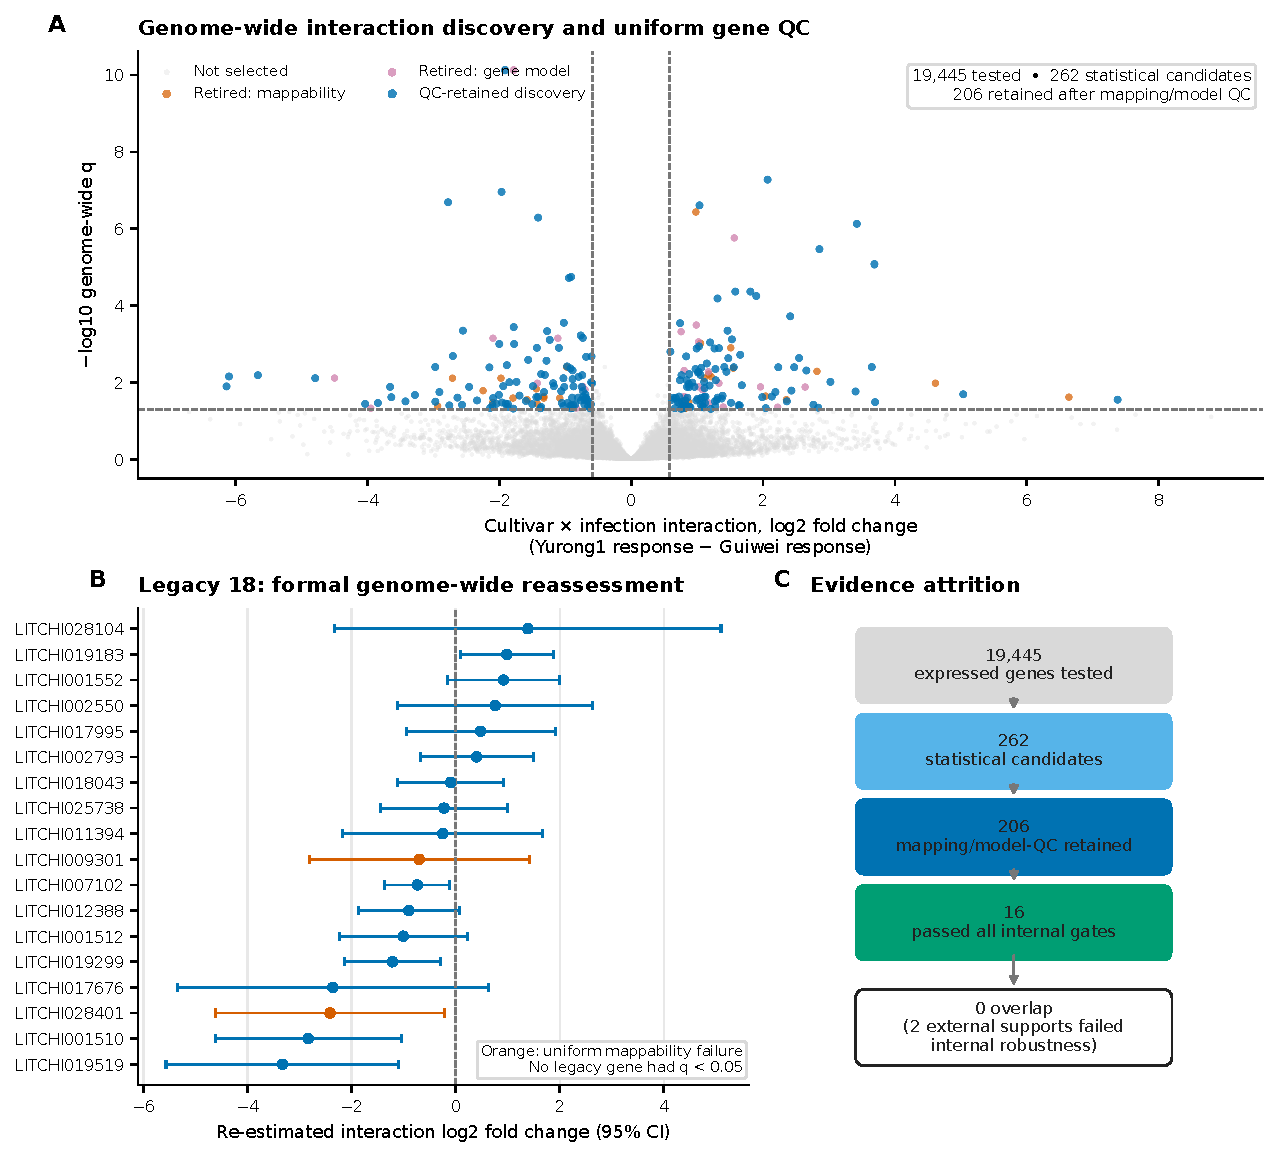
\includegraphics[width=0.98\textwidth]{figure2_discovery_legacy.pdf}
\caption{\textbf{Genome-wide discovery and estimand-aligned assessment of the exploratory candidates.} (A) Cultivar-by-infection interaction effects across 19,445 expressed genes; 262 genes met the statistical threshold and 206 were retained after uniform mapping and gene-model quality control. (B) Genome-wide interaction estimates with 95\% confidence intervals for the 18 exploratory candidates; orange denotes candidates excluded by uniform-mappability control. Their infection responsiveness within each cultivar is evaluated separately in Supplementary S14. (C) Candidate prioritization from tested genes to the internally robust set.}
\label{fig:discovery}
\end{figure}

\subsection{Estimand-aligned follow-up confirms most exploratory infection responses}

The exploratory stage was designed around infection responsiveness within each cultivar. We therefore performed estimand-aligned confirmatory DESeq2 infected-versus-mock fits in Guiwei and Yurong1, with Benjamini--Hochberg adjustment over the same 19,445-gene universe in each contrast (Supplementary S14). Thirteen of the 18 exploratory genes were significant in Guiwei and 16 of 18 in Yurong1 at $\q<0.05$; all 13 Guiwei genes and 15 of the 16 Yurong1 genes also exceeded $|\mathrm{log2FC}|\ge\log_2(1.5)$. These results confirm that most of the original candidates are infection responsive within at least one cultivar. The registered genome-wide analysis addressed the distinct question of whether those responses differed between cultivars (Figure~\ref{fig:discovery}B; Table~\ref{tab:legacy}). No exploratory candidate met the combined interaction threshold. LITCHI001510 reached $\q=0.080$, and the EF-hand calcium-binding gene LITCHI019519 retained a substantial interaction estimate of $-3.33$ ($\q=0.106$); the median interaction \q{} across the 18 candidates was 0.47. Two candidates, LITCHI009301 and LITCHI028401, were not eligible after uniform exon-mappability control because their estimates could not be attributed unambiguously to a single locus. The two analyses therefore provide complementary interpretations: the exploratory set is strongly enriched for within-cultivar infection responses, whereas cultivar-differential response is captured by the genome-wide candidate set described above.

\begin{table}[p]
\centering
\caption{\textbf{Genome-wide interaction estimates for the 18 exploratory-stage candidates.} Effects are re-estimated values for the Yurong1 response minus the Guiwei response (log2 scale). Infection responsiveness within each cultivar is reported in Supplementary S14. The interaction criterion was genome-wide $\q<0.05$ and $|\mathrm{log2FC}|\ge\log_2(1.5)$; none of these candidates met both components.}
\label{tab:legacy}
\footnotesize
\begin{tabular}{@{}llccc@{}}
\toprule
\textbf{Gene} & \textbf{Exploratory annotation} & \textbf{Interaction log2FC (SE)} & \textbf{Genome-wide \q} & \textbf{Mappability} \\
\midrule
LITCHI001510 & Poorly characterized responsive gene & $-2.83$ (0.91) & 0.080 & Pass \\
LITCHI019519 & EF-hand calcium-binding protein & $-3.33$ (1.14) & 0.106 & Pass \\
LITCHI019299 & S-adenosylmethionine-related protein & $-1.21$ (0.47) & 0.175 & Pass \\
LITCHI007102 & Phytosulfokine precursor & $-0.74$ (0.32) & 0.238 & Pass \\
LITCHI019183 & Plant lipid-transfer protein & $+0.99$ (0.45) & 0.273 & Pass \\
LITCHI028401 & Selected interaction candidate & $-2.41$ (1.13) & 0.281 & Not eligible \\
LITCHI012388 & Heat-shock protein 70 & $-0.90$ (0.49) & 0.381 & Pass \\
LITCHI001552 & Cyclase-like stress-related protein & $+0.92$ (0.55) & 0.430 & Pass \\
LITCHI001512 & Poorly characterized responsive gene & $-1.01$ (0.63) & 0.457 & Pass \\
LITCHI017676 & S-adenosylmethionine-related protein & $-2.36$ (1.53) & 0.478 & Pass \\
LITCHI002550 & Cytochrome P450 & $+0.76$ (0.96) & 0.762 & Pass \\
LITCHI028104 & Jacalin-like lectin & $+1.39$ (1.89) & 0.785 & Pass \\
LITCHI002793 & Osmotin/thaumatin-like protein & $+0.41$ (0.55) & 0.786 & Pass \\
LITCHI017995 & Metalloendoproteinase & $+0.48$ (0.73) & 0.812 & Pass \\
LITCHI009301 & Osmotin/thaumatin-like protein & $-0.70$ (1.08) & 0.816 & Not eligible \\
LITCHI025738 & Cyclase-like stress-related protein & $-0.22$ (0.62) & 0.908 & Pass \\
LITCHI011394 & Pathogenesis-related protein & $-0.25$ (0.98) & 0.940 & Pass \\
LITCHI018043 & Plant lipid-transfer protein & $-0.10$ (0.52) & 0.954 & Pass \\
\bottomrule
\end{tabular}
\end{table}

\subsection{Sixteen genes and one pathway passed all internal robustness gates}

Each of the 206 frozen genes was assessed under four predeclared perturbations: independent Salmon-based quantification (196 of 206 retained), edgeR quasi-likelihood testing in place of the primary framework (19 retained), a counts-per-million expression filter (205 retained), and all twelve leave-one-library-out refits (125 retained). Eighteen genes satisfied all four gates jointly, and 16 formed the final internally robust set after observed mapping-sensitivity analysis (Figure~\ref{fig:robust}A). The two statistical frameworks showed exceptionally strong agreement in estimation: interaction effects correlated at Pearson $r=0.995$ across all 19,445 genes and $r=0.999$ across the 206 candidates, all candidate directions agreed, and every candidate had nominal edgeR $P<0.05$. The edgeR gate was selective because the registered rule required genome-wide $\q<0.10$ as well as direction agreement; edgeR retained 24 genes genome-wide at this threshold (10 at $\q<0.05$), compared with 262 under the primary Wald analysis at $\q<0.05$. This calibration difference motivates a transparent evidence hierarchy: 262 statistical candidates, 206 passing quality control, 19 significant in both frameworks, and a stable core of 16 passing the complete registered procedure. At pathway level, circadian rhythm was the single pathway retained across all four complementary gates (competitive and rotation-based testing, leading-edge deletion, and an expression- and length-matched null); the remaining pathways were not retained by the rotation-based test, and maturation was also sensitive to leading-edge deletion.

\begin{figure}[p]
\centering
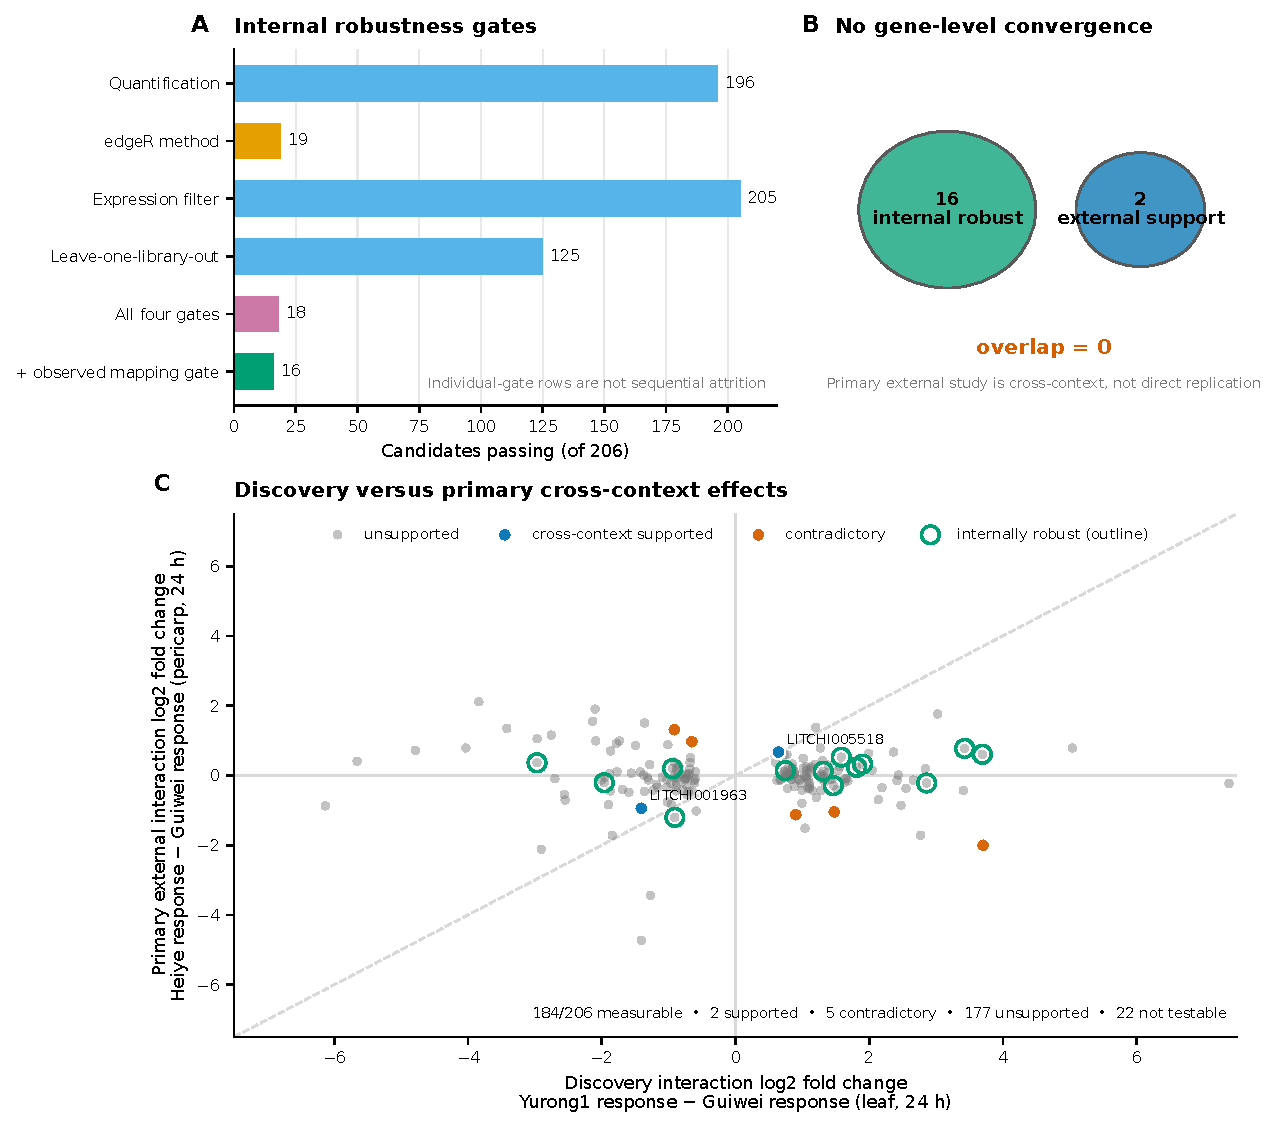
\includegraphics[width=0.98\textwidth]{figure3_robustness_external.pdf}
\caption{\textbf{Internal robustness and context-dependent external responses.} (A) Candidates retained by each predeclared robustness gate, their conjunction, and the additional observed-mapping gate. (B) The 16-gene internally robust set and two genes supported across contexts represent complementary candidate groups; their observed zero overlap is expected for sets of these sizes. (C) Discovery interaction effects against primary cross-context effects (Heiye response minus Guiwei response, pericarp, 24 h), highlighting supported, opposite-direction, and internally robust genes. The diagonal is a visual reference only; equal effects are not expected across different tissues and cultivar contrasts.}
\label{fig:robust}
\end{figure}

\subsection{Cross-context evaluation highlights two supported genes and five response reversals}

The primary external estimand, fixed before unlock, was the resistant-minus-susceptible cultivar-by-infection interaction at 24~h in the PRJNA450886 pericarp time course. Candidate tests used Benjamini--Hochberg adjustment across the full candidate-by-contrast family, an effect threshold of $\log_2(1.5)$, confidence intervals excluding zero, and discovery-direction agreement. Of the 206 frozen genes, 184 were measurable. Two met every criterion for cross-context support: LITCHI005518, an alpha-xylosidase involved in xyloglucan remodeling of the cell wall, and LITCHI001963, an uncharacterized gene with a one-to-one \textit{Oryza} ortholog (Figure~\ref{fig:robust}C; Table~\ref{tab:external}). Five additional genes, including a beta-glucosidase and a Fe(II)/2-oxoglutarate-dependent dioxygenase, met the magnitude and significance criteria in the opposite direction, identifying response reversals across tissue and cultivar contexts. The remaining outcomes were 177 below the prespecified support threshold and 22 not testable. Across the 184 measurable candidates, continuous discovery and external effects were uncorrelated (Pearson $r=-0.05$, 95\% CI $-0.19$ to 0.10; Spearman $\rho=-0.04$), and 95 (51.6\%) shared direction.

The two cross-context-supported genes and the 16 internally robust discovery genes form complementary, non-overlapping groups (Figure~\ref{fig:robust}B). Given sets of 16 and 2 drawn from 206 candidates, the expected overlap under independence is only 0.16 genes and the probability of observing zero overlap is 0.85. The external cohort differs from discovery in tissue (pericarp versus leaf), resistant comparator (Heiye versus Yurong1), and time structure, so the supported genes are notable for transport across contexts, whereas opposite-direction and below-threshold outcomes delineate tissue- or genotype-specific responses. Because Yurong1 and Heiye have not been placed on a common resistance scale relative to Guiwei, this analysis evaluates cross-cultivar response transport rather than direct replication of a resistance phenotype.

\begin{table}[p]
\centering
\caption{\textbf{Cross-context supported genes and response reversals in the primary external evaluation (PRJNA450886, pericarp, 24 h).} Discovery effects are Yurong1-minus-Guiwei interaction log2 fold changes in leaf; external effects are Heiye-minus-Guiwei interaction log2 fold changes in pericarp with 95\% confidence intervals. All \q-values are Benjamini--Hochberg adjusted (discovery: genome-wide; external: across the frozen candidate-by-contrast family).}
\label{tab:external}
\footnotesize
\setlength{\tabcolsep}{2.4pt}
\begin{tabular}{@{}llccccc@{}}
\toprule
\textbf{Gene} & \textbf{Annotation} & \textbf{Disc.\ log2FC} & \textbf{Disc.\ \q} & \textbf{Ext.\ log2FC (95\% CI)} & \textbf{Ext.\ \q} & \textbf{Outcome} \\
\midrule
LITCHI005518 & Alpha-xylosidase 1 & $+0.64$ & 0.025 & $+0.67$ ($+0.32$ to $+1.02$) & 0.007 & Supported \\
LITCHI001963 & Uncharacterized; 1:1 \textit{Oryza} ortholog & $-1.41$ & 0.024 & $-0.94$ ($-1.43$ to $-0.46$) & 0.007 & Supported \\
LITCHI030761 & Caffeoylshikimate esterase & $-0.92$ & 0.040 & $+1.31$ ($+0.78$ to $+1.85$) & 0.0002 & Reversed \\
LITCHI029534 & Thiamine thiazole synthase 2 & $+1.48$ & 0.002 & $-1.04$ ($-1.61$ to $-0.48$) & 0.010 & Reversed \\
LITCHI021860 & Phosphatidylinositol 4-kinase gamma 2 & $-0.65$ & 0.032 & $+0.97$ ($+0.39$ to $+1.54$) & 0.029 & Reversed \\
LITCHI008313 & Beta-glucosidase 44 & $+0.90$ & 0.045 & $-1.12$ ($-1.81$ to $-0.44$) & 0.034 & Reversed \\
LITCHI001700 & Fe(II)/2-OG-dependent dioxygenase 4 & $+3.70$ & 0.033 & $-2.00$ ($-3.24$ to $-0.77$) & 0.035 & Reversed \\
\bottomrule
\end{tabular}
\end{table}

\subsection{The expression signature resolves tissue- and time-dependent infection responses}

The frozen signed signature over the 206 discovery genes captured reproducible, context-dependent infection responses (Figure~\ref{fig:pathways}B). In the generic-transfer study it tracked infection positively in leaf (0.107, $\q=0.0015$) and negatively in fruit ($-0.181$, $\q<0.001$), producing a significant leaf--fruit interaction (0.289, $\q<0.001$). In the primary pericarp time course the score was 0.109 at 24~h (95\% CI $-0.079$ to 0.297, $\q=0.349$) and $-0.240$ at 48~h (95\% CI $-0.428$ to $-0.052$, $\q=0.043$). The signature therefore distinguishes tissue- and time-specific response states rather than serving as a context-invariant marker. At pathway level, the six discovery pathways, including internally robust circadian rhythm, did not meet the external pathway gates in PRJNA450886 (Figure~\ref{fig:pathways}A). The exploratory cohort estimate is reported separately in Figure~S3.

\begin{figure}[p]
\centering
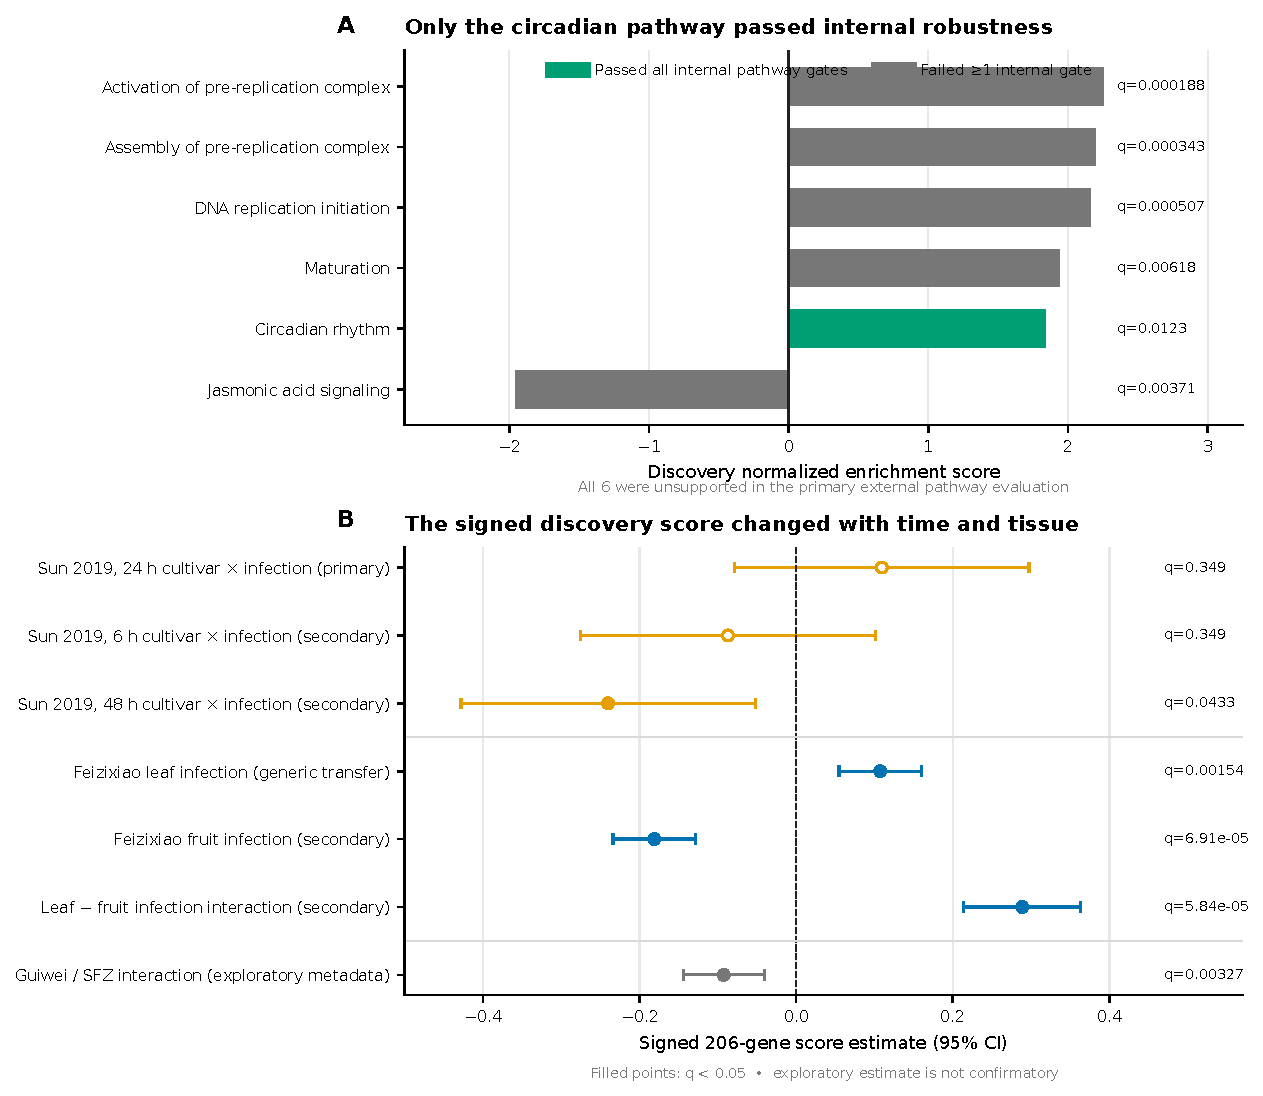
\includegraphics[width=0.92\textwidth]{figure4_pathways_signatures.pdf}
\caption{\textbf{Pathway robustness and context-dependent signature responses.} (A) Discovery normalized enrichment scores for the six frozen pathways; circadian rhythm was retained by all internal gates, whereas none met the primary external criteria. (B) The frozen signed 206-gene signature across six non-exploratory external contrasts; filled points denote $\q<0.05$. The exploratory PRJNA1090613 estimate is shown separately in Figure~S3.}
\label{fig:pathways}
\end{figure}

\subsection{Discovery identifies 225 cultivar-dependent transcript-usage events}

Differential transcript usage was analyzed under a conditional gate registered in advance to ensure interpretable gene- and transcript-level error control. The gate was satisfied, identifying 225 transcript-usage events across 152 genes among 15,790 tested transcripts (Figure~\ref{fig:dtu}A). External follow-up preserved the prespecified role separation (Figure~\ref{fig:dtu}B). In the primary cross-context study, 125 events were measurable but below the support thresholds and 100 were not testable; annotation incompatibilities made the generic-transfer cohort unsuitable for event-level testing. The exploratory cohort yielded four supported and five opposite-direction events, reported descriptively because its metadata could not be standardized. These 225 events provide an internally supported resource for studying cultivar-dependent transcript-level regulation and for future validation with compatible transcript annotations.

\begin{figure}[p]
\centering
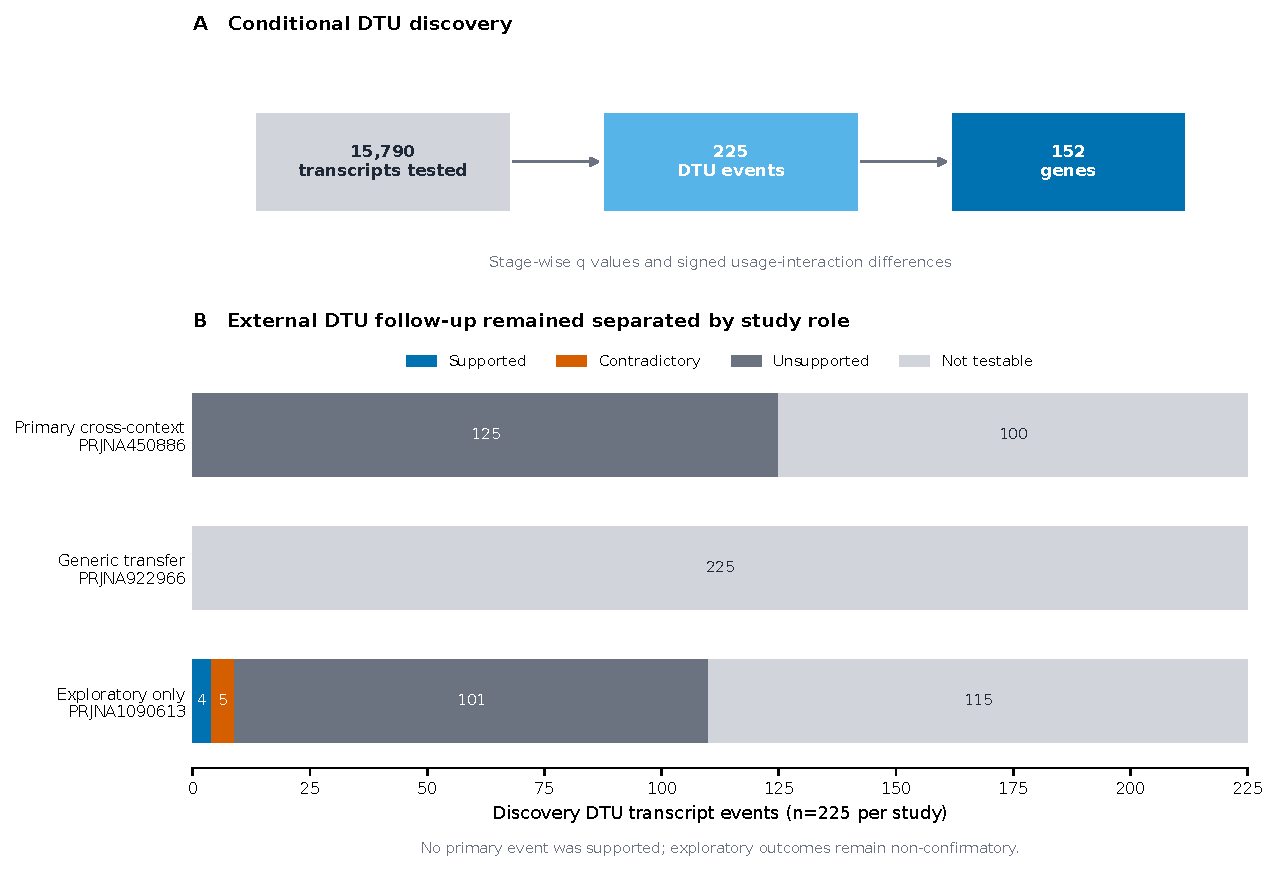
\includegraphics[width=0.98\textwidth]{figure5_transcript_usage.pdf}
\caption{\textbf{Conditional transcript usage.} (A) Discovery gate and event counts. (B) External follow-up of the 225 discovery events, separated by prespecified study role.}
\label{fig:dtu}
\end{figure}

\subsection{Orthogonal analyses refine functional interpretation and reference requirements}

Computational annotation assigned family-level functional labels to 150 of the 206 candidates, enabling interpretation of the prioritized gene sets (Figure~\ref{fig:ortho}A). The registered high-confidence rule additionally required two independent evidence classes, at least 70\% supported coverage, and no architecture conflict. No candidate met this more demanding composite rule, largely because precomputed InterPro domain architectures were unavailable for the 206 proteins in this non-model species; 56 candidates also remained without a family-level label. Registered promoter analysis tested 927 JASPAR plant position-weight matrices in strand-aware 1-kb and 2-kb windows against 100 expression- and GC-matched genomic background sets. Motifs passed in at most 4 of 100 backgrounds, below the prespecified requirement of 80, and none was retained by FIMO sensitivity analysis (Figure~\ref{fig:ortho}B). Small-RNA coherence could not be evaluated because the frozen PmiREN reference contained no exact \textit{Litchi} entries. Together, these results define concrete annotation and reference improvements needed to extend orthogonal evidence in lychee.

A complementary controlled comparison held the published 18-promoter totals, motif strings, scoring rule, and multiplicity correction fixed while changing only the background (Supplementary S15). The 100,000-set randomized-GC rerun closely reproduced the exploratory result. Against 100 expression- and GC-matched genomic promoter sets, MeJA-responsive, TCA, and TC-rich classes remained significant; ARE was replaced by ABRE, so four of seven classes were significant under either strategy while one class changed. This isolates background construction as an influential, but not exclusive, source of variation between the exploratory PlantCARE and registered JASPAR analyses. Interpretation remains conditional on provenance because the exploratory archive did not contain its observed-motif input TSV and canonical-promoter recounting reproduced the published total only for ARE. The controlled analysis consequently supports these motifs as hypotheses for direct regulatory assays rather than evidence of function. Studies reusing an analyzed accession, including the primary external study [5], are retained as prior interpretation rather than counted as independent support.

\begin{figure}[p]
\centering
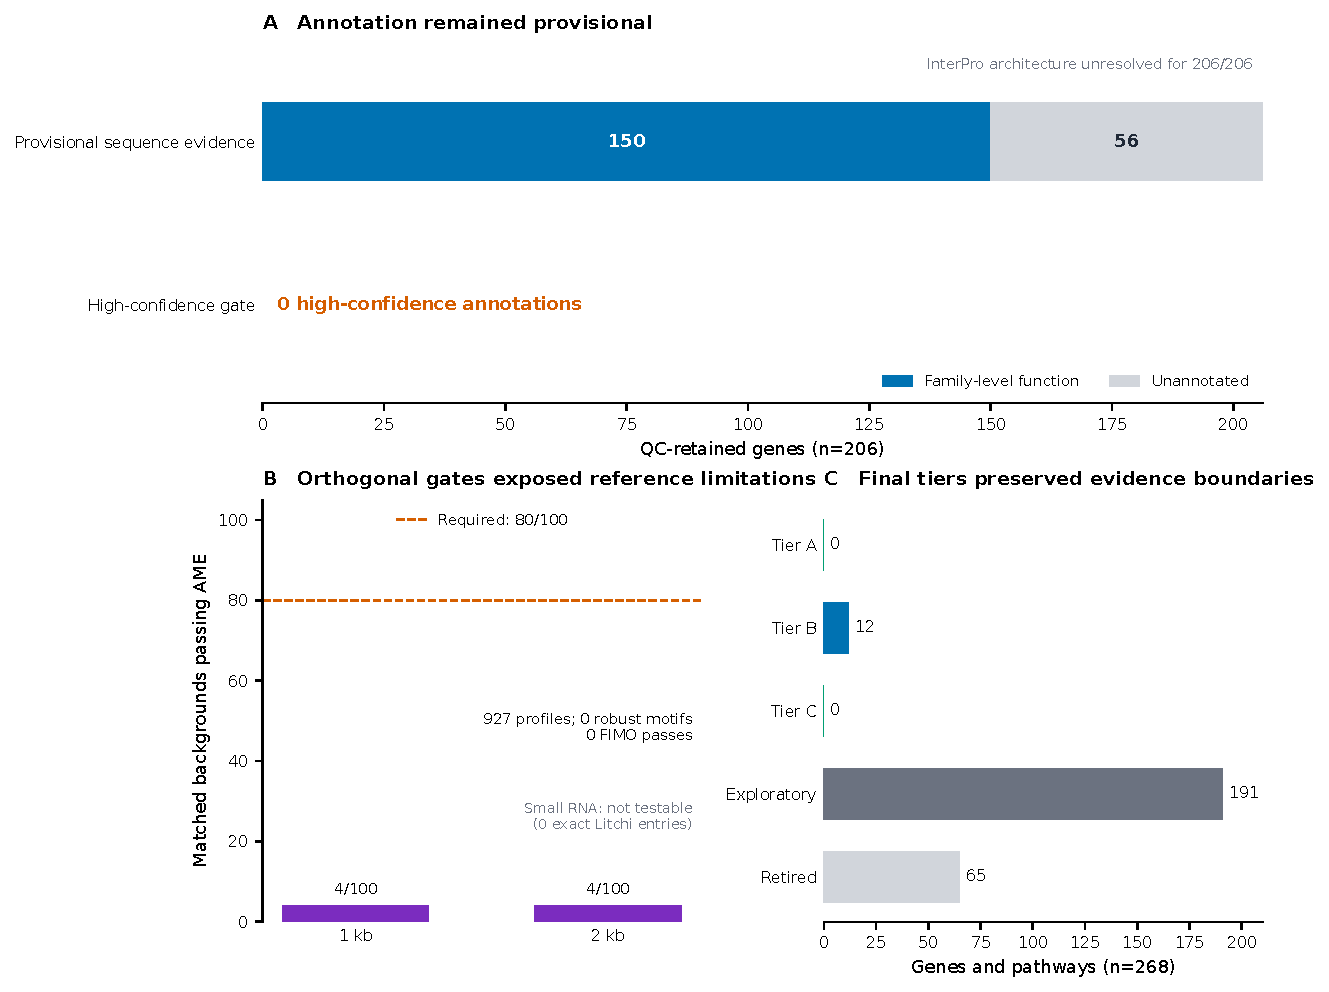
\includegraphics[width=0.98\textwidth]{figure6_orthogonal_tiers.pdf}
\caption{\textbf{Functional annotation, orthogonal analyses, and candidate prioritization.} (A) Annotation status of the 206 QC-retained genes. (B) Registered promoter-motif robustness and the small-RNA reference gate. (C) Deterministic evidence tiers over all 268 frozen entities.}
\label{fig:ortho}
\end{figure}

\subsection{Evidence integration prioritizes twelve internally robust Tier B genes}

The registered rules integrated every evidence layer without discretionary scoring. Applied to 262 statistical gene candidates and 6 pathways, they prioritized 12 genes in Tier B, retained 191 entities for exploratory follow-up, and excluded 65 entities through explicit quality or direction rules (Figure~\ref{fig:ortho}C). Tier A required discovery, complete internal robustness, primary cross-context support, clean mapping and annotation, and an attributable orthogonal class; Tier C required a robust, externally supported pathway. Neither tier was populated under the current data and reference resources. This outcome is partly structural: the small-RNA class was not testable, no motif met the family-wise robustness rule, accession-linked literature was reserved as prior interpretation, and precomputed domain architectures were unavailable for the two-class annotation rule. The tier system therefore concentrates the strongest current expression evidence in Tier B while making the requirements for future promotion explicit.

The 12 Tier B genes are listed in Table~\ref{tab:tierb}. Nine were measurable in the primary external cohort, and all nine retained the discovery direction, although their adjusted external tests did not meet every support criterion. Their annotations converge on carbohydrate and cell-wall metabolism (a phosphomannomutase/phosphoglucomutase, a chloroplastic 1,4-alpha-glucan-branching enzyme, an ERD6-like sugar transporter, and a serine carboxypeptidase), membrane transport (a WAT1-related protein), lipid signaling (a DIR1-like lipid-transfer protein), programmed-cell-death regulation (a BAG-family chaperone regulator), specialized metabolism (cytochrome P450 81Q32), RNA metabolism (ribonuclease J and exonuclease 1), and chromatin-associated regulation (a homeobox-DDT protein), alongside one unannotated gene. Figure~S1 shows the normalized count of every discovery library for these genes, the two cross-context-supported genes, and exploratory highlights LITCHI001510 and LITCHI019519; every cultivar--treatment cell contains all three deposited replicates. Of the 65 excluded entities, 56 were removed by uniform mapping or gene-model control, five showed significant cross-context direction reversal, and four had candidate-level mapping or annotation concerns. These categories remain distinguished in the released tables because a quality-control exclusion and a biologically plausible response reversal have different interpretations.

\begin{table}[t]
\centering
\caption{\textbf{The twelve Tier B genes prioritized by complete internal robustness.} Discovery effects are interaction log2 fold changes (Yurong1 response minus Guiwei response); positive values indicate a stronger infection response in Yurong1. All nine genes measurable in the primary external cohort retained the discovery direction. External columns give the 24-h pericarp estimate with 95\% confidence interval and family-adjusted \q; NM denotes genes not measurable in that cohort.}
\label{tab:tierb}
\footnotesize
\setlength{\tabcolsep}{3pt}
\begin{tabular}{@{}llcccc@{}}
\toprule
\textbf{Gene} & \textbf{Family-level annotation} & \textbf{Disc.\ log2FC} & \textbf{Genome-wide \q} & \textbf{Ext.\ log2FC (95\% CI)} & \textbf{Ext.\ \q} \\
\midrule
LITCHI014613 & Sugar transporter ERD6-like 16 & $+3.69$ & $8.7\times10^{-6}$ & $+0.60$ ($-0.04$ to $+1.25$) & 0.27 \\
LITCHI015982 & WAT1-related protein & $+3.43$ & $7.8\times10^{-7}$ & $+0.77$ ($+0.07$ to $+1.48$) & 0.18 \\
LITCHI005805 & Phosphomannomutase/phosphoglucomutase & $+2.07$ & $5.5\times10^{-8}$ & NM & --- \\
LITCHI028926 & Exonuclease 1 & $+1.90$ & $5.7\times10^{-5}$ & $+0.32$ ($-0.63$ to $+1.28$) & 0.83 \\
LITCHI016077 & Serine carboxypeptidase 24 & $+1.81$ & $4.4\times10^{-5}$ & $+0.23$ ($-1.05$ to $+1.51$) & 0.89 \\
LITCHI013915 & 1,4-alpha-glucan-branching enzyme 3 & $+1.58$ & $4.4\times10^{-5}$ & $+0.53$ ($+0.10$ to $+0.95$) & 0.13 \\
LITCHI021546 & Homeobox-DDT domain protein RLT3 & $+1.31$ & $6.6\times10^{-5}$ & $+0.12$ ($-0.30$ to $+0.54$) & 0.83 \\
LITCHI022605 & Ribonuclease J & $+0.74$ & $2.9\times10^{-4}$ & $+0.14$ ($-0.34$ to $+0.62$) & 0.83 \\
LITCHI028717 & BAG-family chaperone regulator 4 & $-0.91$ & $1.8\times10^{-5}$ & $-1.20$ ($-2.52$ to $+0.12$) & 0.29 \\
LITCHI008721 & Unannotated protein & $-1.91$ & $7.9\times10^{-11}$ & NM & --- \\
LITCHI015740 & Putative lipid-transfer protein DIR1 & $-1.96$ & $1.2\times10^{-7}$ & $-0.21$ ($-1.10$ to $+0.69$) & 0.88 \\
LITCHI010877 & Cytochrome P450 81Q32 & $-2.77$ & $2.1\times10^{-7}$ & NM & --- \\
\bottomrule
\end{tabular}
\end{table}

\subsection{Parametric simulations quantify the interaction effects detectable with three libraries per cell}

The post hoc power analysis simulated negative-binomial counts from the fitted gene-wise means and dispersions while preserving the four-cell discovery design and the 24-h four-cell external design (Figure~S2; Supplementary S18). At each of 12 absolute interaction effects from 0 to 4 log2 units, 100 simulations were run sequentially. Genome-wide discovery used 19,445 tests with 262 injected targets per simulation, matching the observed statistical-candidate prevalence; external analysis adjusted within the 177 frozen genes passing count and dispersion validity filters, with 2 injected targets matching the number of directionally supported genes. Seven additional genes were measurable in the observed 184-gene external contrast but were not fit-eligible for simulation, so the simulated family is reported explicitly. The interpolated effect required for 80\% detection was 2.44 log2FC (5.4-fold) in discovery and 2.11 log2FC (4.3-fold) in external candidate-family analysis. At a true $|$interaction log2FC$|$ of 1.5, detection probabilities were 62.7\% and 74.0\%, respectively. These conditional curves quantify the effects detectable with three deposited libraries per cell and show why below-threshold external results may reflect power as well as biological context.

\section{Discussion}

This analysis identifies a reproducible core of cultivar-dependent transcriptional responses in the lychee--\Pl{} pathosystem and organizes those responses for experimental follow-up. Among 262 genome-wide statistical candidates, 206 passed mapping and gene-model quality control, 19 were significant under both statistical frameworks, and 16 passed the complete registered robustness procedure. Agreement in estimated effects was exceptionally high between DESeq2 and edgeR, and the tier system prioritized 12 genes whose signals were stable across independent quantification, statistical framework, expression filtering, leave-one-library-out analysis, and mapping sensitivity. Two further genes transported across a deliberately different cultivar and tissue context. The estimand-aligned analysis also confirmed infection responsiveness for most of the 18 exploratory genes within Guiwei and Yurong1. Their absence from the genome-wide interaction set reflects the distinction between responsiveness within a cultivar and a difference in response between cultivars, as well as the greater uncertainty of interaction estimation; it does not refute their infection-responsive behavior.

The relationship between the two stages illustrates the value of matching the model to the question. Per-cultivar differential expression and a cultivar-by-infection interaction are different estimands: a gene can respond strongly in one or both cultivars without a precisely estimated difference between those responses. Selection by large observed fold change in a three-replicate contrast also favors estimates with substantial sampling variance. For example, LITCHI019519 retained a large interaction estimate of $-3.33$, but its standard error of 1.14 yielded $\q=0.106$. Uniform-mappability control separately identified two exploratory genes whose locus-specific effects could not be resolved. The combined workflow thus preserves the exploratory genes as well-supported infection-response hypotheses while directing claims about cultivar differences to the genome-wide, quality-controlled candidate set.

The prioritized genes suggest a coherent biological theme centered on cell-wall and carbohydrate dynamics. Tier B includes a phosphomannomutase/phosphoglucomutase, a starch-branching enzyme, an ERD6-like sugar transporter, and a serine carboxypeptidase, while the cross-context-supported set includes an alpha-xylosidase acting on xyloglucan. This qualitative convergence across distinct evidence levels is consistent with prior emphasis on sugar metabolism and cell-wall reinforcement in resistant and susceptible lychee cultivars [5] and with the broader role of apoplastic sugar status and wall remodeling in oomycete interactions. Tier B also includes a DIR1-like lipid-transfer protein, related to a mobile systemic-acquired-resistance signal in \textit{Arabidopsis}, and a BAG-family chaperone regulator from networks that shape plant immunity and immune-associated cell death [9]. Jasmonic acid signaling provides an additional hypothesis: it showed strong discovery enrichment, and jasmonate-associated promoter elements were highlighted in the exploratory analysis, although the pathway was not retained in external testing. These annotations are provisional and were not subjected to a gene-set over-representation test, but their recurrence identifies focused candidates for qPCR and functional studies.

The multi-cohort evaluation reveals pronounced biological context dependence. LITCHI005518, encoding an alpha-xylosidase associated with xyloglucan remodeling, and LITCHI001963 retained their response directions and met all statistical criteria across different tissues and cultivar contrasts. At the broader signature level, a significant leaf--fruit interaction and a time-dependent change between 24 and 48~h show that cultivar-associated infection responses are reorganized across tissue and time. This pattern explains why the internally robust and cross-context-supported sets can be complementary rather than overlapping: with sets of 16 and 2 drawn from 206 genes, zero overlap has probability 0.85 under independence. For breeding applications, the result argues for validating expression candidates in the tissue and developmental window in which they will be deployed, while elevating the two transported genes as especially useful cross-context targets.

The orthogonal analyses add a practical roadmap for extending this resource. Family-level labels were assigned to 150 candidates, but the more stringent two-class annotation rule could not be completed without precomputed InterPro architectures. Similarly, the absence of exact \textit{Litchi} entries in the frozen miRNA reference identifies a concrete barrier to small-RNA integration. The controlled PlantCARE comparison further shows that background definition influences individual motif classes: replacing randomized-GC sequences with expression- and GC-matched genomic promoters exchanged ARE for ABRE while retaining MeJA, TCA, and TC-rich signals. Differences in foreground provenance, motif representation, scoring, and robustness rules also separate this result from the registered JASPAR analysis. Direct regulatory assays and improved species-specific annotation resources are therefore the productive next steps for testing these hypotheses.

The study is bounded by the available public designs. Each cultivar--treatment cell contains three deposited libraries, whose independence at the source-tree, pooling, and extraction levels is not reported; the resulting \q-values are conditional on deposited-library independence. Metadata do not fully specify inoculum form, leaf developmental stage, or wounding, and all quantification uses one reference assembly. The uniform and observed mapping analyses address the clearest reference-related concerns, but residual bias remains possible. The external cohort intentionally differs in tissue, cultivar comparator, and time structure, making a passing result a stringent demonstration of cross-context transport while leaving below-threshold results open to both biological and statistical explanations. Consistent with this distinction, simulations estimated 80\% minimum detectable effects of 2.44 log2FC (5.4-fold) for genome-wide discovery and 2.11 log2FC (4.3-fold) for candidate-family external evaluation. No same-tissue, same-time independent replication cohort is currently available, and the computational candidates have not yet been perturbed experimentally. These limitations define a focused next phase: qPCR of Tier B genes in independently infected Guiwei and Yurong1 material, functional analysis of the alpha-xylosidase and DIR1-like candidates, and promoter--reporter or chromatin-binding assays for regulatory hypotheses.

\section{Conclusions}

This registered multi-cohort analysis defines a robust transcriptional resource for the lychee--\Pl{} pathosystem. It identifies 206 quality-controlled genome-wide interaction candidates, 19 genes significant in two statistical frameworks, a stable core of 16 genes, 12 Tier B candidates spanning cell-wall and carbohydrate metabolism, transport, lipid signaling, chaperone regulation, and RNA metabolism, and two genes supported across an independent tissue and cultivar contrast. The signed expression profile further resolves strong tissue- and time-dependent infection responses, while estimand-aligned analysis confirms within-cultivar responsiveness for most exploratory candidates. By linking every candidate to explicit robustness, context, and annotation evidence, the released tables and workflows provide a reproducible foundation for targeted validation and for developing context-appropriate markers of lychee disease response.

\section{Materials and Methods}

\subsection{Study design, registration, and evidence vocabulary}

The confirmatory stage was governed by a time-stamped protocol, with amendments logged, distributed with the accompanying repository. The registration chronology is as follows. The exploratory stage was completed first, so the discovery dataset had already been analyzed, under different models, before registration. Protocol version 1.0.0 was frozen on 18 August 2026, with its SHA-256 hash (ef668486\ldots) recorded alongside the protocol text, before any confirmatory expression outcome was computed. The amendment log records 20 outcome-blind amendments (clarifications, implementation corrections, and optimizations, all time-stamped before any discovery or external expression outcome was viewed) and 3 post-outcome amendments confined to technical quality control and manifest verification, each marked as such. The primary external study had been published previously [5], and its headline biological conclusions were known to the analyst before registration; dataset roles and all thresholds were nevertheless fixed before any external count matrix was processed. Because all cohorts are public, the staged external unlock is a workflow-enforced computational safeguard, not blinding in the experimental sense. The protocol fixed dataset roles (Table~\ref{tab:roles}), statistical models, discovery and evaluation thresholds, conditional gates, empty-set behavior, and the vocabulary used throughout this paper: \emph{frozen} denotes a computed result fixed at a recorded checkpoint and never modified afterward; \emph{discovery} refers only to the registered genome-wide interaction analysis in PRJNA830488; \emph{robustness} refers only to predeclared sensitivity analyses within that cohort; \emph{cross-context support} denotes a passing frozen external test in a cohort that differs in tissue, comparator, or design, and is never described as replication; and \emph{orthogonal} evidence classes (annotation, motifs, small RNA, literature) are reported separately from expression support and cannot substitute for it. No external outcome could modify frozen discovery membership, signature weights, or thresholds.

\subsection{Exploratory-stage analyses (Stage 1)}

The exploratory stage analyzed the 12 GSE201243 libraries with FastQC v0.11.9 quality control, Trimmomatic v0.39 trimming, TopHat v2.0.12/Bowtie2 v2.2.3 alignment to the SCAU\_Lch\_v2.0 assembly (GCA\_019925255.1), HTSeq v2.0.2 union-mode counting, and DESeq2 v1.42.0 per-cultivar Wald contrasts (design $\sim$ treatment) with Benjamini--Hochberg adjustment at $P<0.05$ [10--15]. Candidate prioritization combined significance, fold-change magnitude, and annotation plausibility; structural, conserved-motif, and promoter analyses used TBtools-II v2.096, MEME v5.5.5, and PlantCARE [16--18]; and the promoter-background comparison tested observed \textit{cis}-element counts in the 18 candidate promoters against 100,000 randomized sets of eighteen 2-kb sequences with lychee-like GC content, scoring exact motifs and reverse complements, with one-sided empirical $P$-values adjusted by Benjamini--Hochberg [19]. The selected-gene interaction contrast was computed as log2FC(Yurong1, infected versus mock) $-$ log2FC(Guiwei, infected versus mock) over the prioritized genes and was explicitly labeled a prioritization effect size rather than a genome-wide test.

\subsection{Data provenance and eligibility}

National Center for Biotechnology Information and Gene Expression Omnibus metadata for all five cohorts were reconciled into a biological-unit registry (Supplementary S1). The original repository preserved accession decisions but not the historical query log, so search coverage was reconstructed retrospectively on 27 August 2026 and is not represented as prospective provenance. A broad NCBI GEO series query returned six records and a corresponding BioProject query returned seven; a narrow SRA cross-check returned 42 experiment-level records. After collapsing the GSE222652 super-series, excluding PRJNA1157370 because it used \textit{Colletotrichum gloeosporioides}, and excluding PRJNA268587/GSE63658 because it studied fruit senescence/storage without \Pl{} inoculation, the five prespecified cohorts remained (Supplementary S16a--b). Because source-tree, pooling, harvest, and extraction independence were not reported for the discovery libraries, all inferential \q-values are conditional on deposited-library independence. The primary model required at least three included libraries in every cultivar-treatment cell.

\subsection{Confirmatory preprocessing and quality gates}

Host (SCAU\_Lch\_v2.0) and pathogen references were combined with prefixed contig names to absorb pathogen-derived reads. Paired reads were checked with FastQC, trimmed with fastp [20], aligned with STAR two-pass mapping [21], counted at the gene level with featureCounts [22], and independently quantified with Salmon [23]. Libraries were excluded if fewer than 10 million read pairs survived trimming or fewer than 40\% of reads aligned uniquely; all 12 discovery libraries passed. GenMap-based exon-uniqueness scores [24] and candidate-level observed-mapping checks were fixed before discovery and used for the uniform mapping and observed mapping-sensitivity gates.

\subsection{Genome-wide discovery model}

DESeq2 [15] fitted gene counts with the design $\sim$ cultivar + treatment + cultivar:treatment (reference levels Guiwei, mock). The primary coefficient, cultivarYurong1:treatmentinfected, estimates the difference in infected-minus-mock response between Yurong1 and Guiwei. Genes required counts of at least 10 in at least three libraries; statistical candidates required genome-wide Benjamini--Hochberg $\q<0.05$ and $|\mathrm{log2FC}|\ge\log_2(1.5)$ [19]. The registered rule tests the point null of zero interaction and applies the effect threshold to the observed estimate. Post hoc sensitivity used DESeq2 with \texttt{lfcThreshold = log2(1.5)} and \texttt{altHypothesis = greaterAbs}, plus apeglm false-sign-or-small $s$-values for the same threshold; neither analysis modified frozen membership. To align the legacy audit with its original estimand, separate post hoc DESeq2 models ($\sim$ treatment) were fitted within Guiwei and Yurong1, using the same count matrix, 19,445-gene universe, and genome-wide Benjamini--Hochberg adjustment within each cultivar. Unshrunken maximum-likelihood estimates are reported throughout; apeglm-shrunken interaction estimates [25] were used only to define the signed signature weights over the 206 frozen genes. Mappability and gene-model metrics were computed for all 19,445 tested genes; as a sensitivity check, recomputing the Benjamini--Hochberg adjustment over only the 13,602 QC-eligible genes rediscovered all 206 frozen candidates plus 12 additional genes, confirming that applying quality control after significance testing was conservative here.

\subsection{Pathway and transcript-usage discovery}

Plant Reactome pathway memberships [26] were transported to lychee through one-to-one reciprocal-best DIAMOND protein matches to \textit{Oryza} [27], and pathway discovery applied the frozen genome-wide interaction statistic to this fixed mapping with camera, roast, and fgsea testing plus leading-edge-deletion and expression/length-matched null gates for robustness [28--30]. Differential transcript usage used Salmon transcript abundances analyzed with DRIMSeq and DEXSeq under stageR stage-wise error control [31--33]; the conditional inferential gate for interpretable two-level error control was registered in advance, and no substitute analysis was permitted had it failed.

\subsection{Internal robustness gates}

Each frozen gene was retested under Salmon-based gene-level quantification, edgeR quasi-likelihood interaction testing [34], a counts-per-million expression filter, and all leave-one-library-out refits, with predeclared criteria combined conjunctively; no additive scoring was used. The Salmon gate required direction agreement and an absolute effect difference of at most 0.5 log2 units; the edgeR analysis used the identical design matrix and interaction coefficient with TMM normalization, robust dispersion estimation (estimateDisp and glmQLFit with robust settings), and glmQLFTest, with Benjamini--Hochberg adjustment computed genome-wide over all 19,445 genes and a gate of genome-wide $\q<0.10$ plus direction agreement; the expression-filter gate refit the primary model after a counts-per-million filter; and the leave-one-library-out gate required direction agreement in all 12 refits and $\q<0.10$ in at least 10 of 12. The observed mapping-sensitivity gate removed candidates whose effect depended on ambiguously mapped reads. Frozen pathways required agreement across camera, roast, leading-edge deletion, and the matched-null comparison.

\subsection{External frozen evaluation}

PRJNA450886 was analyzed with the design $\sim$ cultivar $\times$ treatment $\times$ time, with time encoded as a categorical factor and 24~h as the reference level, so that the cultivar-by-treatment coefficient estimates the 24-h interaction and the three-way terms give the 6-h and 48-h contrasts; the primary estimand was the resistant-minus-susceptible cultivar-by-infection interaction at 24~h, with 6-h and 48-h contrasts secondary. Frozen candidate tests used Benjamini--Hochberg adjustment across the full candidate-by-contrast family, an absolute effect threshold of $\log_2(1.5)$, confidence intervals excluding zero, and discovery-direction agreement; significant opposite-direction responses were recorded separately. PRJNA922966 was analyzed with $\sim$ tissue + treatment + tissue:treatment for generic-transfer tests, and PRJNA1090613 outcomes were confined to exploratory status by protocol. The frozen signed signature was evaluated as a library-level score with the same family-wise adjustment.

\subsection{Annotation, motif, small-RNA, and literature classes}

Representative proteins were chosen by longest coding sequence with lexicographic tie-breaking. Reviewed Swiss-Prot (release 2026\_02) DIAMOND matches [35], targeted InterPro/Pfam domain assignments [36], and one-to-one \textit{Oryza} orthology formed three separate annotation classes; the high-confidence label required at least two classes, at least 70\% supported coverage, and no architecture conflict. Promoter-motif analysis tested 927 JASPAR plant position-weight matrices [37] in strand-aware 1-kb and 2-kb promoter windows against 100 expression- and GC-matched background sets, with AME as the primary test, FIMO as sensitivity [38,39], robustness requiring passes in at least 80 of 100 backgrounds in both windows, and cognate transcription-factor expression required for attribution. The PmiREN bulk archive [40] was audited before small-RNA analysis; because it contained no exact \textit{Litchi} entries, the class was frozen as not testable and no study-derived reference was substituted. Published studies reusing any analyzed accession were registered as prior interpretation. For the post hoc controlled PlantCARE comparison, published observed totals across the 18 legacy promoters were fixed and tested against (i) 100,000 simulated sets of eighteen 2-kb sequences at 34\% GC and (ii) 100 genomic sets of eighteen promoters matched by mean-expression and promoter-GC quintiles with the same seeded minimum-distance rule used by the registered motif pipeline. The six reported motifs and one standard TCA variant, together with reverse complements, were counted and one-sided empirical $P$-values were adjusted across seven classes. The missing archived observed-motif TSV and canonical-promoter recount discrepancies were retained as explicit provenance limitations (Supplementary S15).

\subsection{Simulation-based power analysis}

Negative-binomial parametric simulations used DESeq2 maximum-a-posteriori gene dispersions and fitted sample means from the discovery counts and from the 24-h subset of PRJNA450886. Fitted cultivar and treatment main effects and size factors were retained, background-gene interaction coefficients were set to zero, and equal numbers of positive and negative effects were injected at 12 absolute log2FC values (0, 0.5, 0.75, 1, 1.25, 1.5, 1.75, 2, 2.5, 3, 3.5, 4). Each value had 100 simulations. Discovery injected 262 targets and applied Benjamini--Hochberg correction over 19,445 genes plus the registered effect filter. External simulation injected 2 targets among the 177 frozen genes passing the simulation count and dispersion validity filters and additionally required the prespecified sign and a 95\% interval excluding zero; the observed external table contained 184 measurable genes, seven of which were not fit-eligible for the simulation. Dispersions were treated as known during simulated Wald refits, making the curves conditional parametric power rather than a claim about population-level biological replication. Eighty-percent minimum detectable effects were linearly interpolated between grid points, with expression-quartile curves and Wilson intervals reported in Figure~S2.

\subsection{Tier rules, software versions, and reproducibility}

Tier A required discovery, complete internal robustness, primary cross-context support, clean mapping and annotation, and at least one attributable orthogonal class; Tier B required discovery and complete internal robustness with partial or non-testable primary external evidence; Tier C was reserved for a robust, externally supported pathway. Significant opposite-direction responses and mapping or annotation exclusions were assigned to a separate category, and the rules permitted Tier A to remain unpopulated. All stages ran under Snakemake 9.25.2 workflows [41] enforcing staged discovery, a controlled external unlock, verified cleanup, and SHA-256 manifests over inputs and outputs. Confirmatory executables were FastQC 0.12.1, fastp 1.3.6, STAR 2.7.10b, featureCounts/Subread 2.1.1, Salmon 2.5.1, MEME Suite/AME/FIMO 5.5.9, and DIAMOND 2.2.5; GenMap 1.3.0 is recoverable from the pinned specification although its executable is absent from the reconstructed environment. Statistical work used R 4.3.3/Bioconductor 3.18 with DESeq2 1.42.0, apeglm 1.24.0, edgeR 4.0.16, DRIMSeq 1.30.0, DEXSeq 1.48.0, stageR 1.24.0, and BiocParallel 1.36.0 (Supplementary S17 records the evidence status of every version). The resolved environment, synthetic fixtures, per-figure source data, and amendment log are distributed with the repository. All six main figures are regenerated from frozen result tables by a script that recomputes and asserts every headline count.

\section*{Declarations}

\textbf{Funding:} This work received no external funding. \textbf{Conflicts of interest:} The author declares no conflicts of interest. \textbf{Author contributions:} E.Z. conceived the study, performed all analyses, and wrote the manuscript.

\section*{Data and code availability}

All analyzed data are public: PRJNA830488 (GSE201243, discovery), PRJNA450886 (primary external), PRJNA922966 (GSE222651, generic transfer), PRJNA922965 (GSE222650, small RNA), and PRJNA1090613 (GSE262200, exploratory). The registered protocol, amendment log, complete result tables (all discovery statistics, robustness manifests, external tests, pathway/signature tests, transcript-usage results, annotation and orthogonal evidence, and the contradictory-results file), and the workflow code accompany this repository. Supplementary Tables S1--S18, Figures S1--S3, and tab-separated figure source data are permanently archived under CC BY 4.0 on Zenodo at \url{https://zenodo.org/records/22436625}.

\section*{Supplementary information}

Supplementary tables S1--S18 provide the biological-unit registry, per-library quality control, all 19,445 discovery statistics (including composite-null and false-sign-or-small columns), robustness manifests, all external frozen tests, pathway/signature and transcript-usage results, annotation and orthology evidence, the small-RNA gate, all registered motif-background tests, the evidence registry, script/environment inventory, amendment log, within-cultivar exploratory-candidate assessment (S14), controlled PlantCARE background comparison (S15), reconstructed search queries and eligibility decisions (S16a--b), exact software versions (S17), and power minimum-detectable effects (S18). Figure~S1 shows replicate-level normalized counts, Figure~S2 the conditional power curves, and Figure~S3 the exploratory signature estimate from PRJNA1090613. Every main and supplementary analytical figure has tab-separated source data where applicable.

\setcounter{figure}{0}
\renewcommand{\thefigure}{S\arabic{figure}}

\begin{figure}[p]
\centering
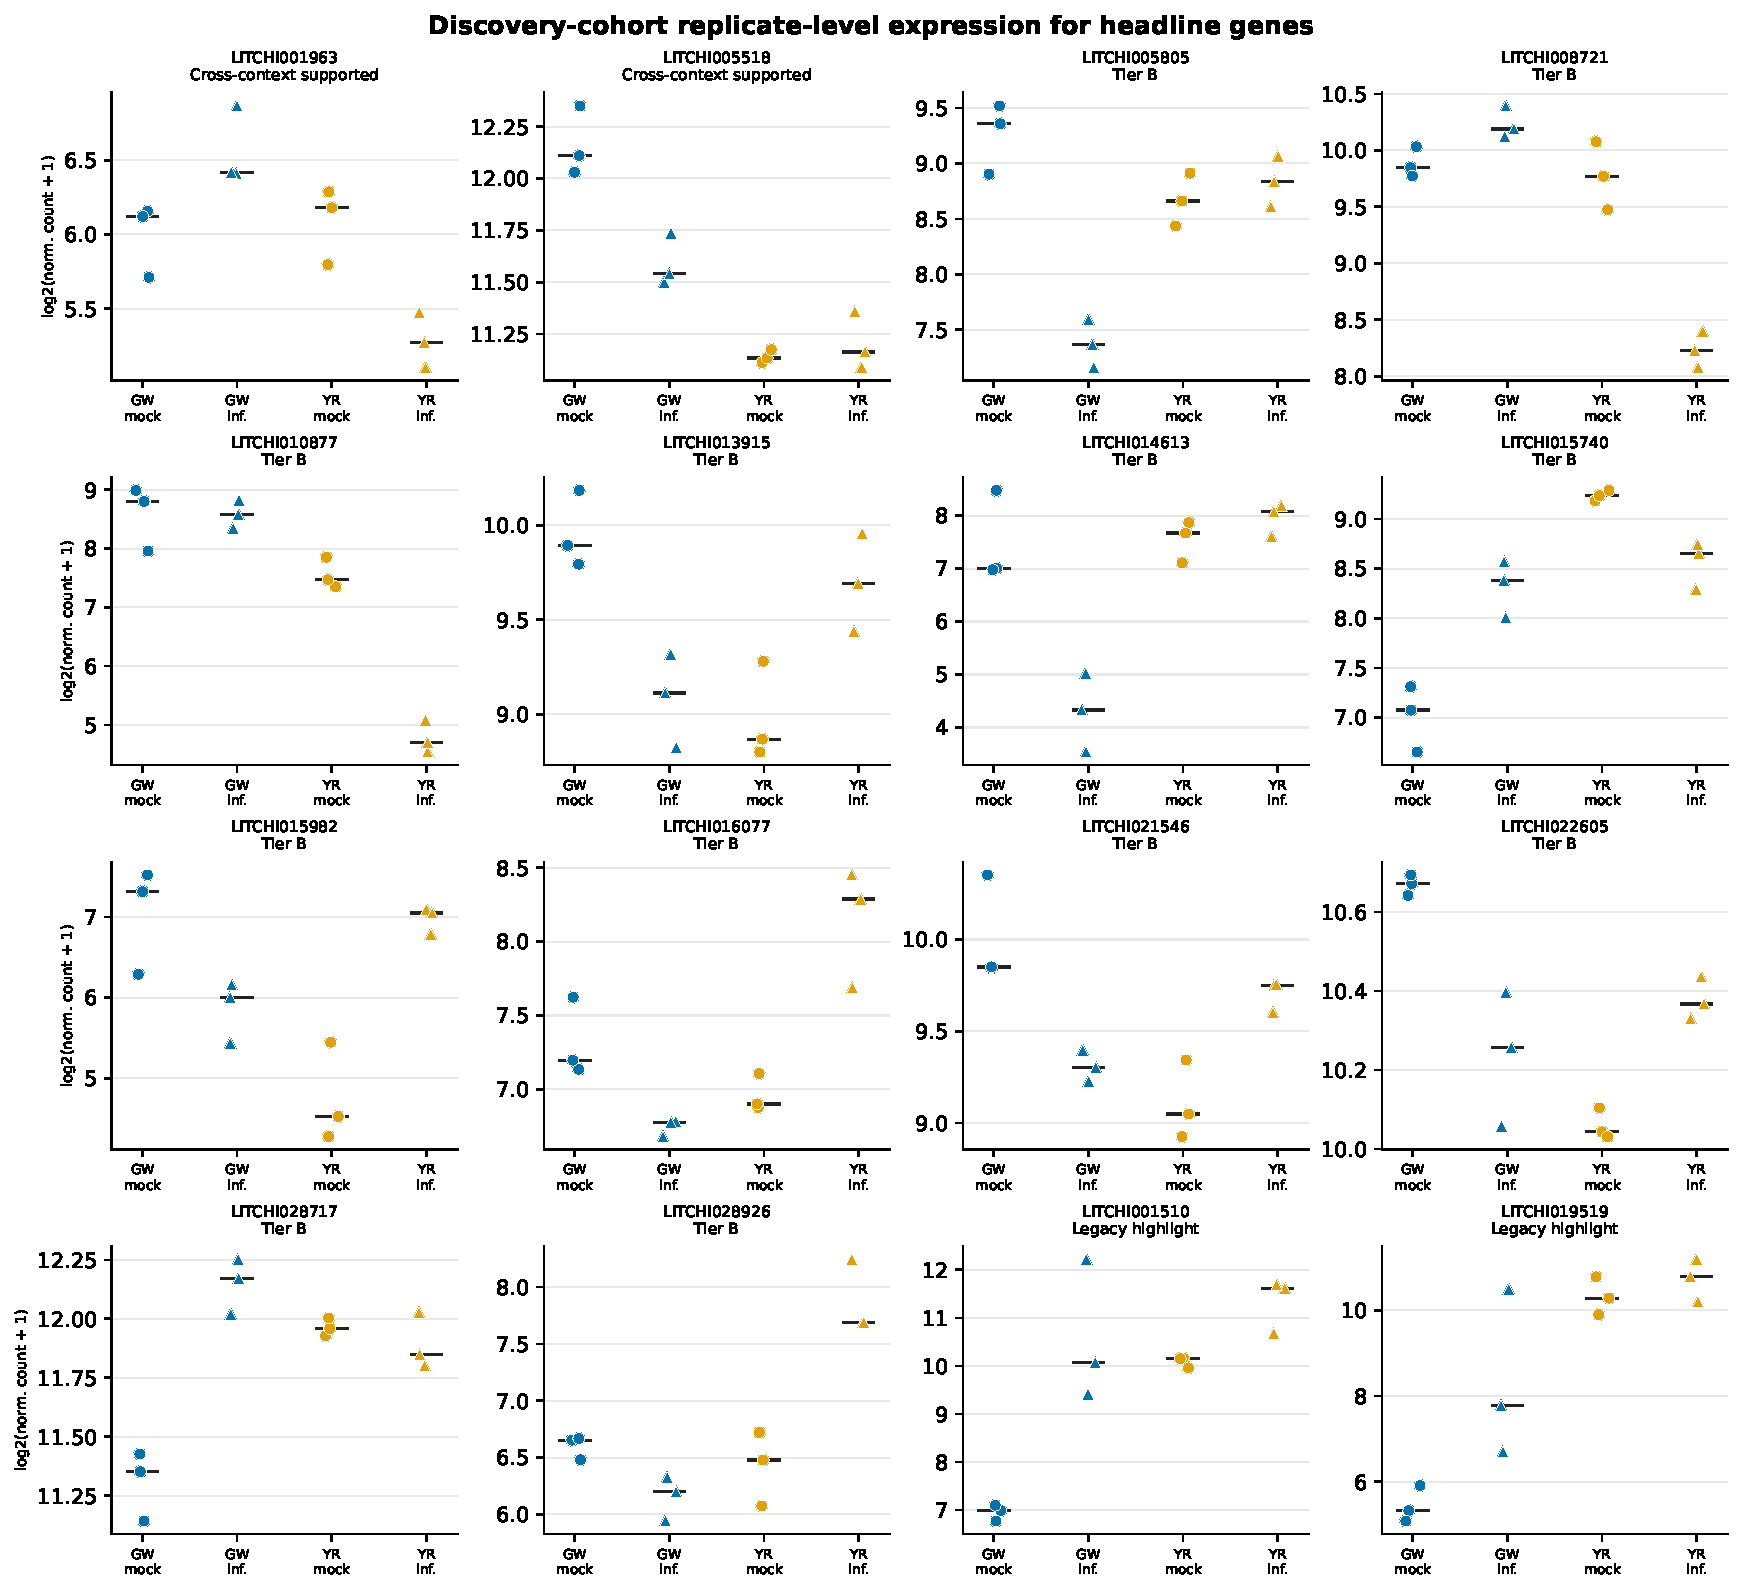
\includegraphics[width=0.98\textwidth]{FigureS1_replicate_level_counts.pdf}
\caption{\textbf{Replicate-level normalized counts for the two cross-context-supported genes, twelve Tier B genes, and two legacy highlights.} Points are individual deposited libraries; bars show cultivar-treatment medians.}
\label{fig:supp-counts}
\end{figure}

\begin{figure}[p]
\centering
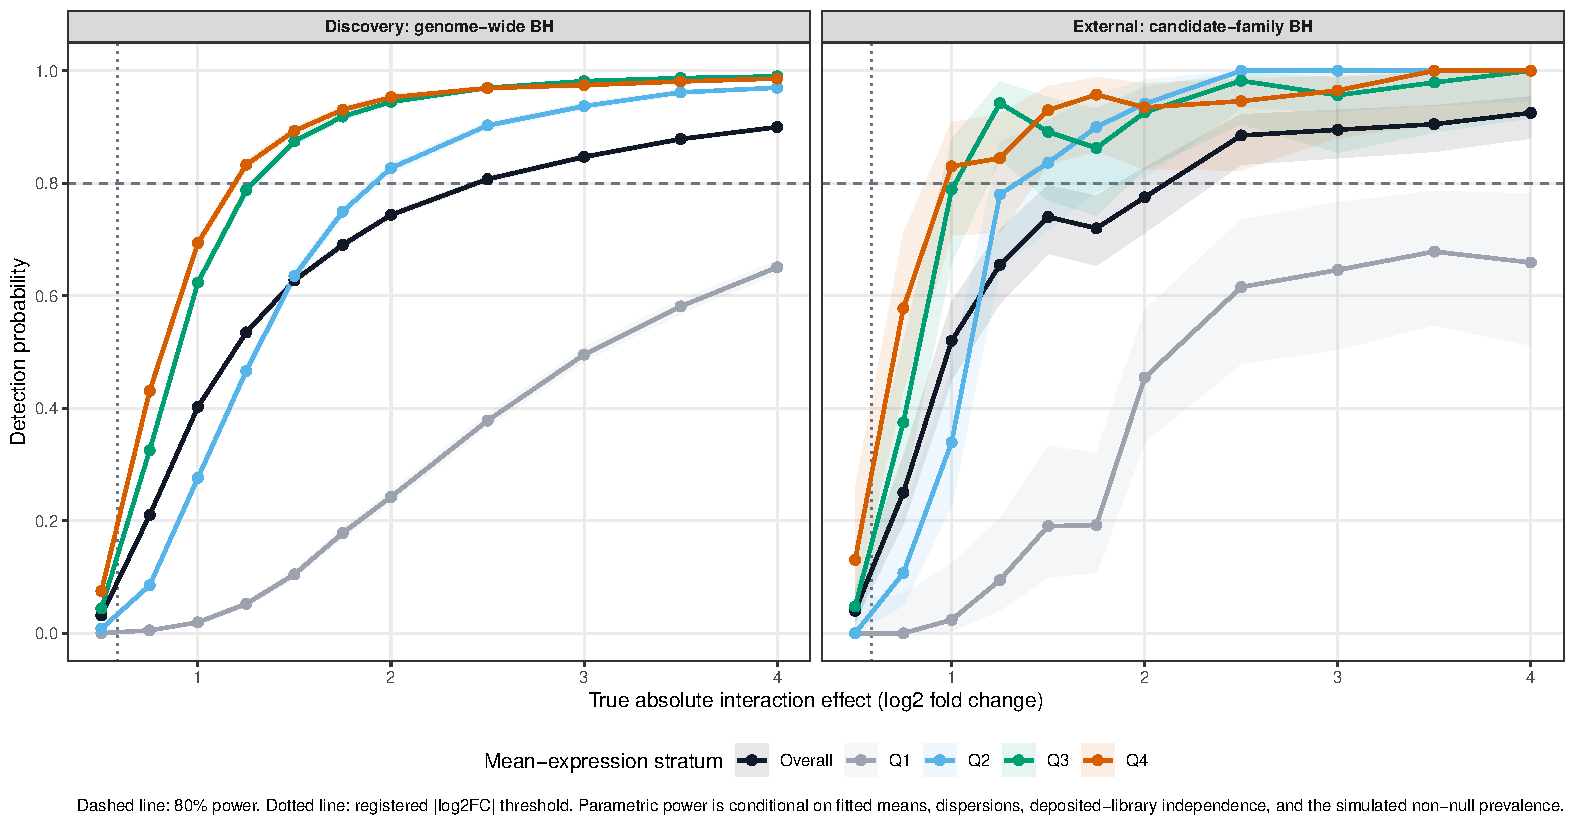
\includegraphics[width=0.9\textwidth]{FigureS2_power_analysis.pdf}
\caption{\textbf{Parametric detection probability for cultivar-by-infection effects under genome-wide discovery and candidate-family external adjustment.} Curves show the overall result and mean-expression quartiles; the dashed line marks 80\% power.}
\label{fig:supp-power}
\end{figure}

\begin{figure}[p]
\centering
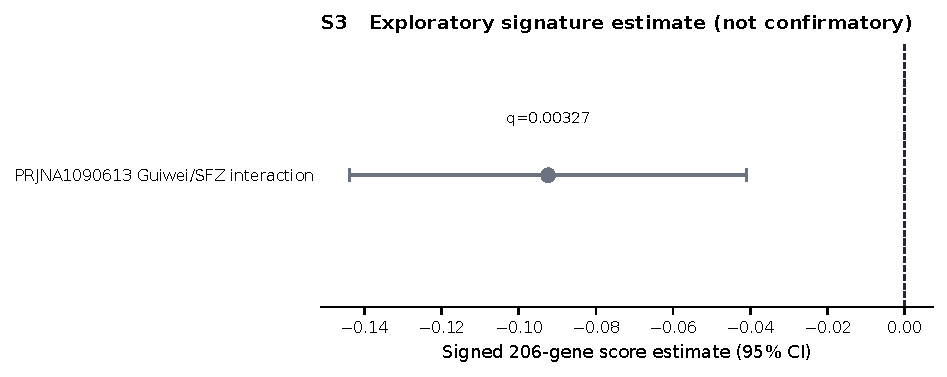
\includegraphics[width=0.7\textwidth]{figureS3_exploratory_signature.pdf}
\caption{\textbf{Exploratory PRJNA1090613 signed-signature estimate,} shown separately because cohort metadata did not support its inclusion in the confirmatory evaluation.}
\label{fig:supp-exploratory}
\end{figure}

\clearpage

\section*{References}
\begin{enumerate}[itemsep=1pt,leftmargin=1.6em]
\item Morton JF. Lychee. In: Fruits of Warm Climates. Winterville: Creative Resource Systems; 1987. p.~249--259.
\item Sun J, Gao Z, Zhang X, Zou X, Cao L, Wang J. Transcriptome analysis of \textit{Phytophthora litchii} reveals pathogenicity arsenals and confirms taxonomic status. PLoS ONE. 2017;12:e0178245.
\item Yi C, Jiang Y, Shi J, Qu H, Xue S, Duan X, et al. ATP-regulation of antioxidant properties and phenolics in litchi fruit during browning and pathogen infection process. Food Chemistry. 2010;118:42--47.
\item Hu G, Feng J, Xiang X, Wang J, Saloj\"arvi J, Liu C, et al. Two divergent haplotypes from a highly heterozygous lychee genome suggest independent domestication events for early and late-maturing cultivars. Nature Genetics. 2022;54:73--83.
\item Sun J, Cao L, Li H, Wang G, Wang S, Li F, et al. Early responses given distinct tactics to infection of \textit{Peronophythora litchii} in susceptible and resistant litchi cultivar. Scientific Reports. 2019;9:2810.
\item Liu H, Yan Q, Jiang Y, Shi F, Chen J, Cai C, et al. Identification of LcCDPKs and analysis of their expression patterns in response to downy mildew stresses in lychee. Journal of Fruit Science. 2023;40:442--456.
\item Li P, Li W, Zhou X, Situ J, Xie L, Xi P, et al. \textit{Peronophythora litchii} RXLR effector PlAvh202 destabilizes a host ethylene biosynthesis enzyme. Plant Physiology. 2023;193:756--774.
\item National Center for Biotechnology Information. GEO accession GSE201243. \url{https://www.ncbi.nlm.nih.gov/geo/query/acc.cgi?acc=GSE201243}.
\item Berka M, Kopeck\'a R, Berkov\'a V, Brzobohat\'y B, \v{C}ern\'y M. Regulation of heat shock proteins 70 and their role in plant immunity. Journal of Experimental Botany. 2022;73:1894--1909.
\item Andrews S. FastQC: a quality control tool for high throughput sequence data. Babraham Bioinformatics; 2010.
\item Bolger AM, Lohse M, Usadel B. Trimmomatic: a flexible trimmer for Illumina sequence data. Bioinformatics. 2014;30:2114--2120.
\item Kim D, Pertea G, Trapnell C, Pimentel H, Kelley R, Salzberg SL. TopHat2: accurate alignment of transcriptomes in the presence of insertions, deletions and gene fusions. Genome Biology. 2013;14:R36.
\item Anders S, Pyl PT, Huber W. HTSeq---a Python framework to work with high-throughput sequencing data. Bioinformatics. 2015;31:166--169.
\item Genome Warehouse. \textit{Litchi chinensis} SCAU\_Lch\_v2.0 assembly (GCA\_019925255.1). National Genomics Data Center, China National Center for Bioinformation.
\item Love MI, Huber W, Anders S. Moderated estimation of fold change and dispersion for RNA-seq data with DESeq2. Genome Biology. 2014;15:550.
\item Chen C, Chen H, Zhang Y, Thomas HR, Frank MH, He Y, et al. TBtools: an integrative toolkit developed for interactive analyses of big biological data. Molecular Plant. 2020;13:1194--1202.
\item Bailey TL, Elkan C. Fitting a mixture model by expectation maximization to discover motifs in biopolymers. In: Proceedings of the Second International Conference on Intelligent Systems for Molecular Biology. Menlo Park: AAAI Press; 1994. p.~28--36.
\item Lescot M, D\'ehais P, Thijs G, Marchal K, Moreau Y, Van de Peer Y, et al. PlantCARE, a database of plant cis-acting regulatory elements and a portal to tools for in silico analysis of promoter sequences. Nucleic Acids Research. 2002;30:325--327.
\item Benjamini Y, Hochberg Y. Controlling the false discovery rate: a practical and powerful approach to multiple testing. Journal of the Royal Statistical Society, Series B. 1995;57:289--300.
\item Chen S, Zhou Y, Chen Y, Gu J. fastp: an ultra-fast all-in-one FASTQ preprocessor. Bioinformatics. 2018;34:i884--i890.
\item Dobin A, Davis CA, Schlesinger F, Drenkow J, Zaleski C, Jha S, et al. STAR: ultrafast universal RNA-seq aligner. Bioinformatics. 2013;29:15--21.
\item Liao Y, Smyth GK, Shi W. featureCounts: an efficient general purpose program for assigning sequence reads to genomic features. Bioinformatics. 2014;30:923--930.
\item Patro R, Duggal G, Love MI, Irizarry RA, Kingsford C. Salmon provides fast and bias-aware quantification of transcript expression. Nature Methods. 2017;14:417--419.
\item Pockrandt C, Alzamel M, Iliopoulos CS, Reinert K. GenMap: ultra-fast computation of genome mappability. Bioinformatics. 2020;36:3687--3692.
\item Zhu A, Ibrahim JG, Love MI. Heavy-tailed prior distributions for sequence count data: removing the noise and preserving large differences. Bioinformatics. 2019;35:2084--2092.
\item Naithani S, Gupta P, Preece J, D'Eustachio P, Elser J, Garg P, et al. Plant Reactome knowledgebase: empowering plant pathway exploration and OMICS data analysis. Nucleic Acids Research. 2024;52:D1538--D1547.
\item Buchfink B, Xie C, Huson DH. Fast and sensitive protein alignment using DIAMOND. Nature Methods. 2015;12:59--60.
\item Wu D, Smyth GK. Camera: a competitive gene set test accounting for inter-gene correlation. Nucleic Acids Research. 2012;40:e133.
\item Wu D, Lim E, Vaillant F, Asselin-Labat ML, Visvader JE, Smyth GK. ROAST: rotation gene set tests for complex microarray experiments. Bioinformatics. 2010;26:2176--2182.
\item Korotkevich G, Sukhov V, Budin N, Shpak B, Artyomov MN, Sergushichev A. Fast gene set enrichment analysis. bioRxiv. 2021:060012.
\item Nowicka M, Robinson MD. DRIMSeq: a Dirichlet-multinomial framework for multivariate count outcomes in genomics. F1000Research. 2016;5:1356.
\item Anders S, Reyes A, Huber W. Detecting differential usage of exons from RNA-seq data. Genome Research. 2012;22:2008--2017.
\item Van den Berge K, Soneson C, Robinson MD, Clement L. stageR: a general stage-wise method for controlling the gene-level false discovery rate in differential expression and differential transcript usage. Genome Biology. 2017;18:151.
\item Robinson MD, McCarthy DJ, Smyth GK. edgeR: a Bioconductor package for differential expression analysis of digital gene expression data. Bioinformatics. 2010;26:139--140.
\item The UniProt Consortium. UniProt: the Universal Protein Knowledgebase in 2023. Nucleic Acids Research. 2023;51:D523--D531.
\item Jones P, Binns D, Chang HY, Fraser M, Li W, McAnulla C, et al. InterProScan 5: genome-scale protein function classification. Bioinformatics. 2014;30:1236--1240.
\item Rauluseviciute I, Riudavets-Puig R, Blanc-Mathieu R, Castro-Mondragon JA, Ferenc K, Kumar V, et al. JASPAR 2024: 20th anniversary of the open-access database of transcription factor binding profiles. Nucleic Acids Research. 2024;52:D174--D182.
\item McLeay RC, Bailey TL. Motif enrichment analysis: a unified framework and an evaluation on ChIP data. BMC Bioinformatics. 2010;11:165.
\item Grant CE, Bailey TL, Noble WS. FIMO: scanning for occurrences of a given motif. Bioinformatics. 2011;27:1017--1018.
\item Guo Z, Kuang Z, Wang Y, Zhao Y, Tao Y, Cheng C, et al. PmiREN: a comprehensive encyclopedia of plant miRNAs. Nucleic Acids Research. 2020;48:D1114--D1121.
\item M\"older F, Jablonski KP, Letcher B, Hall MB, Tomkins-Tinch CH, Sochat V, et al. Sustainable data analysis with Snakemake. F1000Research. 2021;10:33.
\end{enumerate}

\end{document}
